% Options for packages loaded elsewhere
\PassOptionsToPackage{unicode}{hyperref}
\PassOptionsToPackage{hyphens}{url}
%
\documentclass[
]{article}
\usepackage{lmodern}
\usepackage{amssymb,amsmath}
\usepackage{ifxetex,ifluatex}
\ifnum 0\ifxetex 1\fi\ifluatex 1\fi=0 % if pdftex
  \usepackage[T1]{fontenc}
  \usepackage[utf8]{inputenc}
  \usepackage{textcomp} % provide euro and other symbols
\else % if luatex or xetex
  \usepackage{unicode-math}
  \defaultfontfeatures{Scale=MatchLowercase}
  \defaultfontfeatures[\rmfamily]{Ligatures=TeX,Scale=1}
\fi
% Use upquote if available, for straight quotes in verbatim environments
\IfFileExists{upquote.sty}{\usepackage{upquote}}{}
\IfFileExists{microtype.sty}{% use microtype if available
  \usepackage[]{microtype}
  \UseMicrotypeSet[protrusion]{basicmath} % disable protrusion for tt fonts
}{}
\makeatletter
\@ifundefined{KOMAClassName}{% if non-KOMA class
  \IfFileExists{parskip.sty}{%
    \usepackage{parskip}
  }{% else
    \setlength{\parindent}{0pt}
    \setlength{\parskip}{6pt plus 2pt minus 1pt}}
}{% if KOMA class
  \KOMAoptions{parskip=half}}
\makeatother
\usepackage{xcolor}
\IfFileExists{xurl.sty}{\usepackage{xurl}}{} % add URL line breaks if available
\IfFileExists{bookmark.sty}{\usepackage{bookmark}}{\usepackage{hyperref}}
\hypersetup{
  pdftitle={Data 621 Homework 3: Boston Crime Rates},
  pdfauthor={Tommy Jenkins, Violeta Stoyanova, Todd Weigel, Peter Kowalchuk, Eleanor R-Secoquian, Anthony Pagan},
  hidelinks,
  pdfcreator={LaTeX via pandoc}}
\urlstyle{same} % disable monospaced font for URLs
\usepackage[margin=1in]{geometry}
\usepackage{color}
\usepackage{fancyvrb}
\newcommand{\VerbBar}{|}
\newcommand{\VERB}{\Verb[commandchars=\\\{\}]}
\DefineVerbatimEnvironment{Highlighting}{Verbatim}{commandchars=\\\{\}}
% Add ',fontsize=\small' for more characters per line
\usepackage{framed}
\definecolor{shadecolor}{RGB}{248,248,248}
\newenvironment{Shaded}{\begin{snugshade}}{\end{snugshade}}
\newcommand{\AlertTok}[1]{\textcolor[rgb]{0.94,0.16,0.16}{#1}}
\newcommand{\AnnotationTok}[1]{\textcolor[rgb]{0.56,0.35,0.01}{\textbf{\textit{#1}}}}
\newcommand{\AttributeTok}[1]{\textcolor[rgb]{0.77,0.63,0.00}{#1}}
\newcommand{\BaseNTok}[1]{\textcolor[rgb]{0.00,0.00,0.81}{#1}}
\newcommand{\BuiltInTok}[1]{#1}
\newcommand{\CharTok}[1]{\textcolor[rgb]{0.31,0.60,0.02}{#1}}
\newcommand{\CommentTok}[1]{\textcolor[rgb]{0.56,0.35,0.01}{\textit{#1}}}
\newcommand{\CommentVarTok}[1]{\textcolor[rgb]{0.56,0.35,0.01}{\textbf{\textit{#1}}}}
\newcommand{\ConstantTok}[1]{\textcolor[rgb]{0.00,0.00,0.00}{#1}}
\newcommand{\ControlFlowTok}[1]{\textcolor[rgb]{0.13,0.29,0.53}{\textbf{#1}}}
\newcommand{\DataTypeTok}[1]{\textcolor[rgb]{0.13,0.29,0.53}{#1}}
\newcommand{\DecValTok}[1]{\textcolor[rgb]{0.00,0.00,0.81}{#1}}
\newcommand{\DocumentationTok}[1]{\textcolor[rgb]{0.56,0.35,0.01}{\textbf{\textit{#1}}}}
\newcommand{\ErrorTok}[1]{\textcolor[rgb]{0.64,0.00,0.00}{\textbf{#1}}}
\newcommand{\ExtensionTok}[1]{#1}
\newcommand{\FloatTok}[1]{\textcolor[rgb]{0.00,0.00,0.81}{#1}}
\newcommand{\FunctionTok}[1]{\textcolor[rgb]{0.00,0.00,0.00}{#1}}
\newcommand{\ImportTok}[1]{#1}
\newcommand{\InformationTok}[1]{\textcolor[rgb]{0.56,0.35,0.01}{\textbf{\textit{#1}}}}
\newcommand{\KeywordTok}[1]{\textcolor[rgb]{0.13,0.29,0.53}{\textbf{#1}}}
\newcommand{\NormalTok}[1]{#1}
\newcommand{\OperatorTok}[1]{\textcolor[rgb]{0.81,0.36,0.00}{\textbf{#1}}}
\newcommand{\OtherTok}[1]{\textcolor[rgb]{0.56,0.35,0.01}{#1}}
\newcommand{\PreprocessorTok}[1]{\textcolor[rgb]{0.56,0.35,0.01}{\textit{#1}}}
\newcommand{\RegionMarkerTok}[1]{#1}
\newcommand{\SpecialCharTok}[1]{\textcolor[rgb]{0.00,0.00,0.00}{#1}}
\newcommand{\SpecialStringTok}[1]{\textcolor[rgb]{0.31,0.60,0.02}{#1}}
\newcommand{\StringTok}[1]{\textcolor[rgb]{0.31,0.60,0.02}{#1}}
\newcommand{\VariableTok}[1]{\textcolor[rgb]{0.00,0.00,0.00}{#1}}
\newcommand{\VerbatimStringTok}[1]{\textcolor[rgb]{0.31,0.60,0.02}{#1}}
\newcommand{\WarningTok}[1]{\textcolor[rgb]{0.56,0.35,0.01}{\textbf{\textit{#1}}}}
\usepackage{longtable,booktabs}
% Correct order of tables after \paragraph or \subparagraph
\usepackage{etoolbox}
\makeatletter
\patchcmd\longtable{\par}{\if@noskipsec\mbox{}\fi\par}{}{}
\makeatother
% Allow footnotes in longtable head/foot
\IfFileExists{footnotehyper.sty}{\usepackage{footnotehyper}}{\usepackage{footnote}}
\makesavenoteenv{longtable}
\usepackage{graphicx,grffile}
\makeatletter
\def\maxwidth{\ifdim\Gin@nat@width>\linewidth\linewidth\else\Gin@nat@width\fi}
\def\maxheight{\ifdim\Gin@nat@height>\textheight\textheight\else\Gin@nat@height\fi}
\makeatother
% Scale images if necessary, so that they will not overflow the page
% margins by default, and it is still possible to overwrite the defaults
% using explicit options in \includegraphics[width, height, ...]{}
\setkeys{Gin}{width=\maxwidth,height=\maxheight,keepaspectratio}
% Set default figure placement to htbp
\makeatletter
\def\fps@figure{htbp}
\makeatother
\setlength{\emergencystretch}{3em} % prevent overfull lines
\providecommand{\tightlist}{%
  \setlength{\itemsep}{0pt}\setlength{\parskip}{0pt}}
\setcounter{secnumdepth}{-\maxdimen} % remove section numbering
\usepackage{booktabs}
\usepackage{longtable}
\usepackage{array}
\usepackage{multirow}
\usepackage{wrapfig}
\usepackage{float}
\usepackage{colortbl}
\usepackage{pdflscape}
\usepackage{tabu}
\usepackage{threeparttable}
\usepackage{threeparttablex}
\usepackage[normalem]{ulem}
\usepackage{makecell}
\usepackage{xcolor}

\title{Data 621 Homework 3: Boston Crime Rates}
\author{Tommy Jenkins, Violeta Stoyanova, Todd Weigel, Peter Kowalchuk, Eleanor
R-Secoquian, Anthony Pagan}
\date{October, 2019}

\begin{document}
\maketitle

\hypertarget{overview}{%
\section{OVERVIEW}\label{overview}}

In this homework assignment, we will explore, analyze and model a data
set containing information on crime for various neighborhoods of a major
city. Each record has a response variable indicating whether or not the
crime rate is above the median crime rate (1) or not (0).

\hypertarget{objective}{%
\subsection{Objective:}\label{objective}}

The objective is to build a binary logistic regression model on the
training data set to predict whether the neighborhood will be at risk
for high crime levels.

\hypertarget{data-exploration}{%
\section{DATA EXPLORATION}\label{data-exploration}}

\hypertarget{data-summary}{%
\subsection{Data Summary}\label{data-summary}}

The dataset consists of two data files: training and evaluation. The
training dataset contains 13 columns, while the evaluation dataset
contains 12. The evaluation dataset is missing column target which
represend our responce variable and defines whether the crime rate is
above the median crime rate (1) or not (0). We will start by exploring
the training data set since it will be the one used to generate the
regression model.

First we see that all data is numeric. The dataset does contain one
dummy variable to identify if the property borders the Charles River (1)
or not (0).

An important aspect of any dataset is to determine how much, if any,
data is missing. We look at all the variables to see which if any have
missing data. We look at the basic descriptive statistics as well as the
missing data and their percentages:

\begin{verbatim}
##         vars   n   mean     sd median trimmed    mad    min    max  range  skew
## zn         1 466  11.58  23.36   0.00    5.35   0.00   0.00 100.00 100.00  2.18
## indus      2 466  11.11   6.85   9.69   10.91   9.34   0.46  27.74  27.28  0.29
## chas       3 466   0.07   0.26   0.00    0.00   0.00   0.00   1.00   1.00  3.34
## nox        4 466   0.55   0.12   0.54    0.54   0.13   0.39   0.87   0.48  0.75
## rm         5 466   6.29   0.70   6.21    6.26   0.52   3.86   8.78   4.92  0.48
## age        6 466  68.37  28.32  77.15   70.96  30.02   2.90 100.00  97.10 -0.58
## dis        7 466   3.80   2.11   3.19    3.54   1.91   1.13  12.13  11.00  1.00
## rad        8 466   9.53   8.69   5.00    8.70   1.48   1.00  24.00  23.00  1.01
## tax        9 466 409.50 167.90 334.50  401.51 104.52 187.00 711.00 524.00  0.66
## ptratio   10 466  18.40   2.20  18.90   18.60   1.93  12.60  22.00   9.40 -0.75
## lstat     11 466  12.63   7.10  11.35   11.88   7.07   1.73  37.97  36.24  0.91
## medv      12 466  22.59   9.24  21.20   21.63   6.00   5.00  50.00  45.00  1.08
## target    13 466   0.49   0.50   0.00    0.49   0.00   0.00   1.00   1.00  0.03
##         kurtosis   se na_count na_count_perc
## zn          3.81 1.08        0             0
## indus      -1.24 0.32        0             0
## chas        9.15 0.01        0             0
## nox        -0.04 0.01        0             0
## rm          1.54 0.03        0             0
## age        -1.01 1.31        0             0
## dis         0.47 0.10        0             0
## rad        -0.86 0.40        0             0
## tax        -1.15 7.78        0             0
## ptratio    -0.40 0.10        0             0
## lstat       0.50 0.33        0             0
## medv        1.37 0.43        0             0
## target     -2.00 0.02        0             0
\end{verbatim}

\begin{verbatim}
##      zn   indus    chas     nox      rm     age     dis     rad     tax ptratio 
##       0       0       0       0       0       0       0       0       0       0 
##   lstat    medv  target 
##       0       0       0
\end{verbatim}

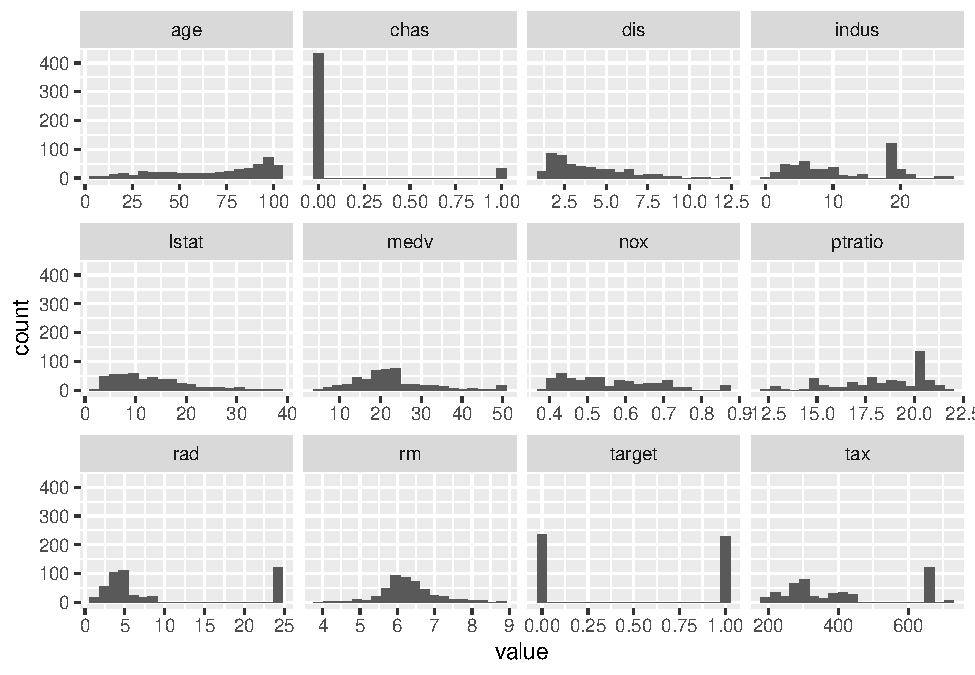
\includegraphics{Data621-Group1-HW3-FINAL_files/figure-latex/unnamed-chunk-7-1.pdf}

\begin{verbatim}
##   zn indus chas   nox    rm   age    dis rad tax ptratio lstat medv target
## 1  0 19.58    0 0.605 7.929  96.2 2.0459   5 403    14.7  3.70 50.0      1
## 2  0 19.58    1 0.871 5.403 100.0 1.3216   5 403    14.7 26.82 13.4      1
## 3  0 18.10    0 0.740 6.485 100.0 1.9784  24 666    20.2 18.85 15.4      1
## 4 30  4.93    0 0.428 6.393   7.8 7.0355   6 300    16.6  5.19 23.7      0
## 5  0  2.46    0 0.488 7.155  92.2 2.7006   3 193    17.8  4.82 37.9      0
## 6  0  8.56    0 0.520 6.781  71.3 2.8561   5 384    20.9  7.67 26.5      0
\end{verbatim}

\hypertarget{missing-and-invalid-data}{%
\subsection{Missing and Invalid Data}\label{missing-and-invalid-data}}

No missing data was found in the dataset.

With missing data assessed, we can look into the data in more detail. To
visualize this we plot histograms for each data. Several predictors like
dist, chas, rad, zn and tax are not normally distributed and noticable
outliers.

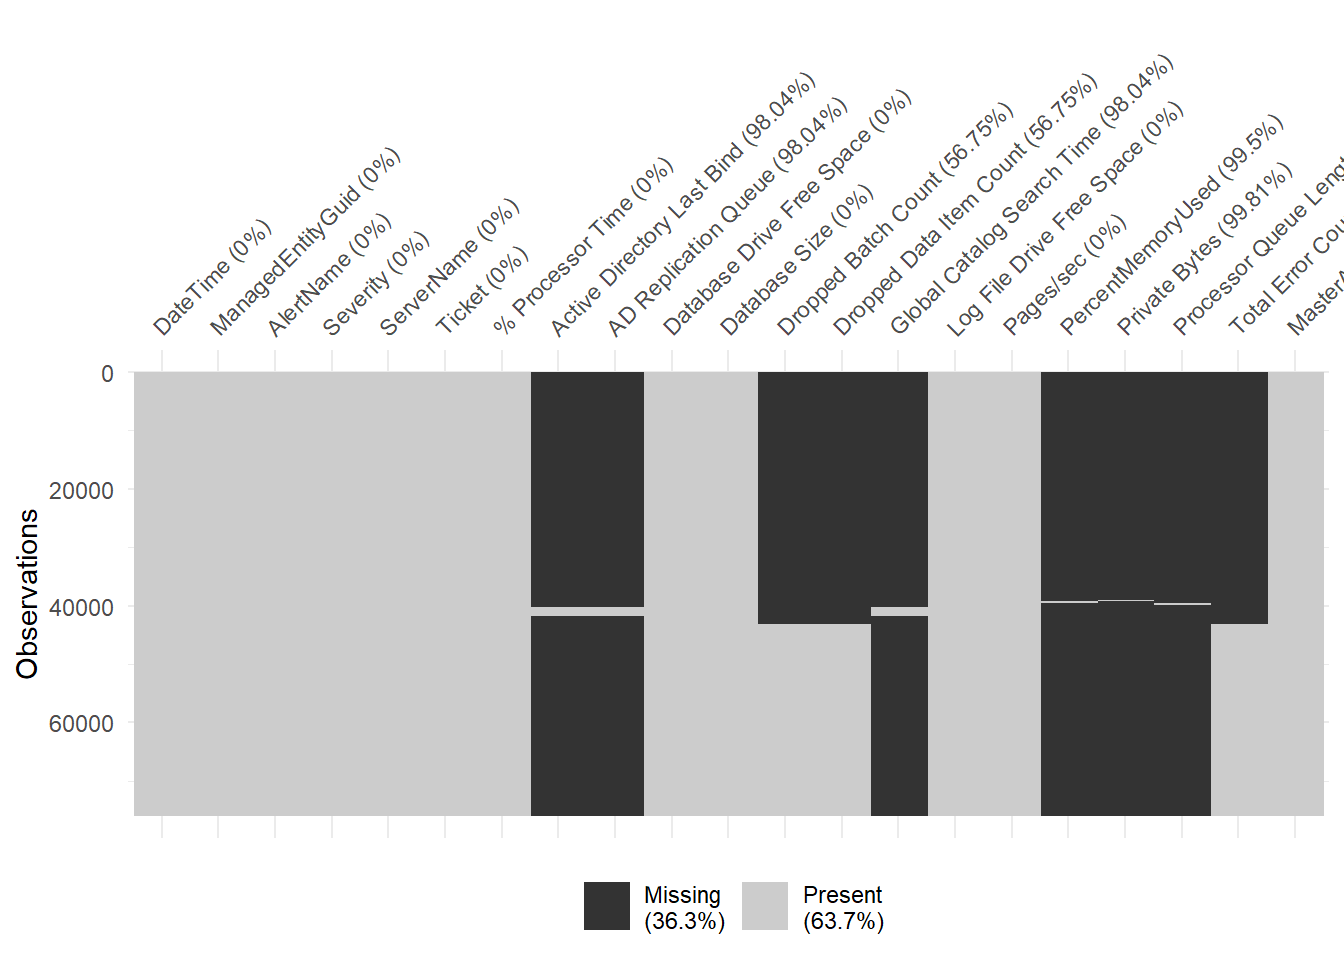
\includegraphics{Data621-Group1-HW3-FINAL_files/figure-latex/unnamed-chunk-8-1.pdf}
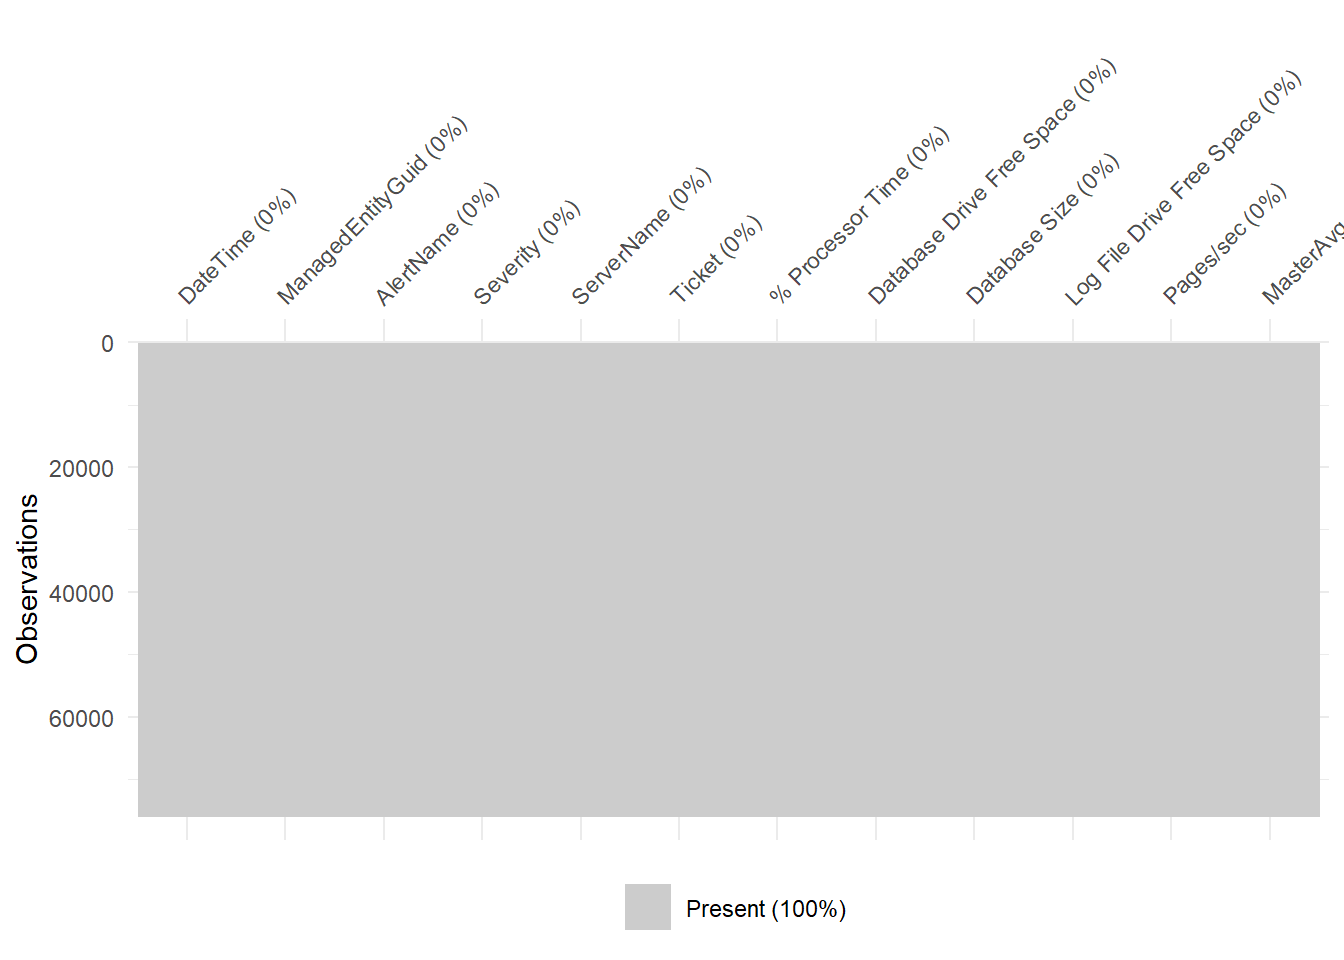
\includegraphics{Data621-Group1-HW3-FINAL_files/figure-latex/unnamed-chunk-8-2.pdf}

\hypertarget{data-preparation}{%
\section{DATA PREPARATION}\label{data-preparation}}

\hypertarget{fix-missing-values}{%
\subsection{Fix missing values}\label{fix-missing-values}}

No data was found missing.

\hypertarget{mathematical-transformations.}{%
\subsection{Mathematical
transformations.}\label{mathematical-transformations.}}

\textbf{Box Cox} The Box Cox transformation tries to transform
non-normal data into a normal distribution. This transformation attemps
to estimate the \(\lambda\) for Y. With the exception of tax, all
predictors have either no transformation extimate or were given a fudge
value of 0.

\begin{verbatim}
## $zn
## Box-Cox Transformation
## 
## 466 data points used to estimate Lambda
## 
## Input data summary:
##    Min. 1st Qu.  Median    Mean 3rd Qu.    Max. 
##    0.00    0.00    0.00   11.58   16.25  100.00 
## 
## Lambda could not be estimated; no transformation is applied
## 
## 
## $indus
## Box-Cox Transformation
## 
## 466 data points used to estimate Lambda
## 
## Input data summary:
##    Min. 1st Qu.  Median    Mean 3rd Qu.    Max. 
##   0.460   5.145   9.690  11.105  18.100  27.740 
## 
## Largest/Smallest: 60.3 
## Sample Skewness: 0.289 
## 
## Estimated Lambda: 0.4 
## 
## 
## $chas
## Box-Cox Transformation
## 
## 466 data points used to estimate Lambda
## 
## Input data summary:
##    Min. 1st Qu.  Median    Mean 3rd Qu.    Max. 
## 0.00000 0.00000 0.00000 0.07082 0.00000 1.00000 
## 
## Lambda could not be estimated; no transformation is applied
## 
## 
## $nox
## Box-Cox Transformation
## 
## 466 data points used to estimate Lambda
## 
## Input data summary:
##    Min. 1st Qu.  Median    Mean 3rd Qu.    Max. 
##  0.3890  0.4480  0.5380  0.5543  0.6240  0.8710 
## 
## Largest/Smallest: 2.24 
## Sample Skewness: 0.746 
## 
## Estimated Lambda: -0.9 
## 
## 
## $rm
## Box-Cox Transformation
## 
## 466 data points used to estimate Lambda
## 
## Input data summary:
##    Min. 1st Qu.  Median    Mean 3rd Qu.    Max. 
##   3.863   5.887   6.210   6.291   6.630   8.780 
## 
## Largest/Smallest: 2.27 
## Sample Skewness: 0.479 
## 
## Estimated Lambda: 0.2 
## 
## 
## $age
## Box-Cox Transformation
## 
## 466 data points used to estimate Lambda
## 
## Input data summary:
##    Min. 1st Qu.  Median    Mean 3rd Qu.    Max. 
##    2.90   43.88   77.15   68.37   94.10  100.00 
## 
## Largest/Smallest: 34.5 
## Sample Skewness: -0.578 
## 
## Estimated Lambda: 1.3 
## 
## 
## $dis
## Box-Cox Transformation
## 
## 466 data points used to estimate Lambda
## 
## Input data summary:
##    Min. 1st Qu.  Median    Mean 3rd Qu.    Max. 
##   1.130   2.101   3.191   3.796   5.215  12.127 
## 
## Largest/Smallest: 10.7 
## Sample Skewness: 0.999 
## 
## Estimated Lambda: -0.1 
## With fudge factor, Lambda = 0 will be used for transformations
## 
## 
## $rad
## Box-Cox Transformation
## 
## 466 data points used to estimate Lambda
## 
## Input data summary:
##    Min. 1st Qu.  Median    Mean 3rd Qu.    Max. 
##    1.00    4.00    5.00    9.53   24.00   24.00 
## 
## Largest/Smallest: 24 
## Sample Skewness: 1.01 
## 
## Estimated Lambda: -0.2 
## With fudge factor, Lambda = 0 will be used for transformations
## 
## 
## $tax
## Box-Cox Transformation
## 
## 466 data points used to estimate Lambda
## 
## Input data summary:
##    Min. 1st Qu.  Median    Mean 3rd Qu.    Max. 
##   187.0   281.0   334.5   409.5   666.0   711.0 
## 
## Largest/Smallest: 3.8 
## Sample Skewness: 0.659 
## 
## Estimated Lambda: -0.5 
## 
## 
## $ptratio
## Box-Cox Transformation
## 
## 466 data points used to estimate Lambda
## 
## Input data summary:
##    Min. 1st Qu.  Median    Mean 3rd Qu.    Max. 
##    12.6    16.9    18.9    18.4    20.2    22.0 
## 
## Largest/Smallest: 1.75 
## Sample Skewness: -0.754 
## 
## Estimated Lambda: 2 
## 
## 
## $lstat
## Box-Cox Transformation
## 
## 466 data points used to estimate Lambda
## 
## Input data summary:
##    Min. 1st Qu.  Median    Mean 3rd Qu.    Max. 
##   1.730   7.043  11.350  12.631  16.930  37.970 
## 
## Largest/Smallest: 21.9 
## Sample Skewness: 0.906 
## 
## Estimated Lambda: 0.2 
## 
## 
## $medv
## Box-Cox Transformation
## 
## 466 data points used to estimate Lambda
## 
## Input data summary:
##    Min. 1st Qu.  Median    Mean 3rd Qu.    Max. 
##    5.00   17.02   21.20   22.59   25.00   50.00 
## 
## Largest/Smallest: 10 
## Sample Skewness: 1.08 
## 
## Estimated Lambda: 0.2 
## 
## 
## $target
## Box-Cox Transformation
## 
## 466 data points used to estimate Lambda
## 
## Input data summary:
##    Min. 1st Qu.  Median    Mean 3rd Qu.    Max. 
##  0.0000  0.0000  0.0000  0.4914  1.0000  1.0000 
## 
## Lambda could not be estimated; no transformation is applied
\end{verbatim}

\hypertarget{variable-creation-removal}{%
\subsection{Variable Creation /
Removal}\label{variable-creation-removal}}

To determine how we can combine variables to create new one we start by
looking at a correlation plot. The plot and cor funtion lists nox, age,
rad,tax and indus as the strongest postively correlated predictors,
while rad and distance are the strongest negatively correlated
predictors.

\begin{verbatim}
##          indus       chas       nox         rm       age        dis       rad
## [1,] 0.6048507 0.08004187 0.7261062 -0.1525533 0.6301062 -0.6186731 0.6281049
##            tax   ptratio    lstat       medv target
## [1,] 0.6111133 0.2508489 0.469127 -0.2705507      1
\end{verbatim}

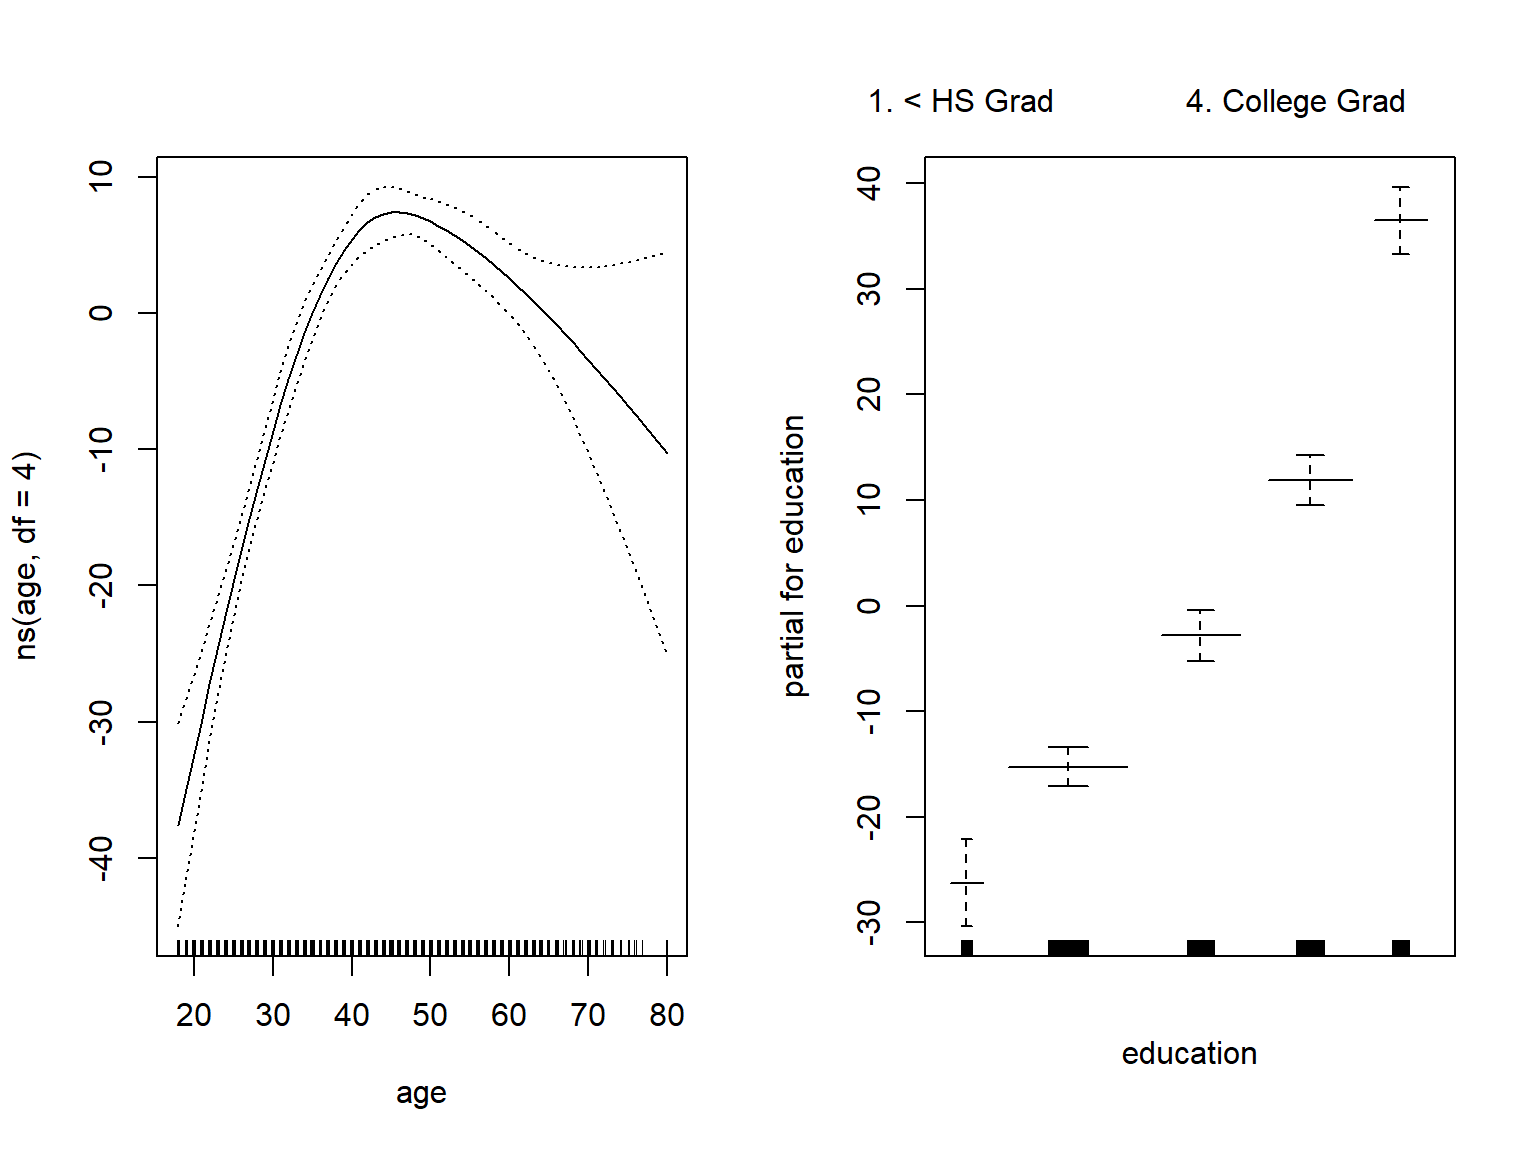
\includegraphics{Data621-Group1-HW3-FINAL_files/figure-latex/unnamed-chunk-11-1.pdf}

\hypertarget{build-models}{%
\section{BUILD MODELS}\label{build-models}}

\hypertarget{general-regression-model-1}{%
\subsubsection{General regression Model
1}\label{general-regression-model-1}}

We start by building a model with all the predictors in the dataset. The
below is referred to as Model 1 later in the document.

\begin{verbatim}
## 
## Call:
## glm(formula = target ~ ., family = binomial(link = "logit"), 
##     data = crimeTrain)
## 
## Deviance Residuals: 
##     Min       1Q   Median       3Q      Max  
## -1.8464  -0.1445  -0.0017   0.0029   3.4665  
## 
## Coefficients:
##               Estimate Std. Error z value Pr(>|z|)    
## (Intercept) -40.822934   6.632913  -6.155 7.53e-10 ***
## zn           -0.065946   0.034656  -1.903  0.05706 .  
## indus        -0.064614   0.047622  -1.357  0.17485    
## chas          0.910765   0.755546   1.205  0.22803    
## nox          49.122297   7.931706   6.193 5.90e-10 ***
## rm           -0.587488   0.722847  -0.813  0.41637    
## age           0.034189   0.013814   2.475  0.01333 *  
## dis           0.738660   0.230275   3.208  0.00134 ** 
## rad           0.666366   0.163152   4.084 4.42e-05 ***
## tax          -0.006171   0.002955  -2.089  0.03674 *  
## ptratio       0.402566   0.126627   3.179  0.00148 ** 
## lstat         0.045869   0.054049   0.849  0.39608    
## medv          0.180824   0.068294   2.648  0.00810 ** 
## ---
## Signif. codes:  0 '***' 0.001 '**' 0.01 '*' 0.05 '.' 0.1 ' ' 1
## 
## (Dispersion parameter for binomial family taken to be 1)
## 
##     Null deviance: 645.88  on 465  degrees of freedom
## Residual deviance: 192.05  on 453  degrees of freedom
## AIC: 218.05
## 
## Number of Fisher Scoring iterations: 9
\end{verbatim}

The Summary of this model shows several predictor are not relevant. We
build a second model without these predictors.

\begin{verbatim}
## 
## Call:
## glm(formula = target ~ nox + age + dis + rad + tax + ptratio + 
##     medv, family = binomial(link = "logit"), data = crimeTrain)
## 
## Deviance Residuals: 
##      Min        1Q    Median        3Q       Max  
## -2.01059  -0.19744  -0.01371   0.00402   3.06424  
## 
## Coefficients:
##               Estimate Std. Error z value Pr(>|z|)    
## (Intercept) -36.824228   5.858405  -6.286 3.26e-10 ***
## nox          42.338378   6.639207   6.377 1.81e-10 ***
## age           0.031882   0.010693   2.982 0.002867 ** 
## dis           0.429555   0.171849   2.500 0.012433 *  
## rad           0.701767   0.139426   5.033 4.82e-07 ***
## tax          -0.008237   0.002534  -3.250 0.001153 ** 
## ptratio       0.376575   0.108912   3.458 0.000545 ***
## medv          0.093653   0.033556   2.791 0.005255 ** 
## ---
## Signif. codes:  0 '***' 0.001 '**' 0.01 '*' 0.05 '.' 0.1 ' ' 1
## 
## (Dispersion parameter for binomial family taken to be 1)
## 
##     Null deviance: 645.88  on 465  degrees of freedom
## Residual deviance: 203.45  on 458  degrees of freedom
## AIC: 219.45
## 
## Number of Fisher Scoring iterations: 9
\end{verbatim}

\begin{verbatim}
## [1] 1
\end{verbatim}

\begin{verbatim}
## [1] 1
\end{verbatim}

The new model has a slightly higher AIC which would tells us the first
model is slightly less complex. For the 2 data sets p-value = 1 -
pchisq(deviance, degrees of freedom) are 1. The Null hypothesis is still
supported.

\hypertarget{aic-step-method-model-2}{%
\subsubsection{AIC Step Method Model 2}\label{aic-step-method-model-2}}

Another way of selecting which predictors to use in the model is by
calculating the AIC of the model. This metric is similar to the adjusted
R-square of a model in that it penalizes models with more predictors
over simpler model with few predictors. We use Stepwise function in r to
find the lowest AIC with different predictors.

\begin{verbatim}
## Start:  AIC=218.05
## target ~ zn + indus + chas + nox + rm + age + dis + rad + tax + 
##     ptratio + lstat + medv
## 
##           Df Deviance    AIC
## - rm       1   192.71 216.71
## - lstat    1   192.77 216.77
## - chas     1   193.53 217.53
## - indus    1   193.99 217.99
## <none>         192.05 218.05
## - tax      1   196.59 220.59
## - zn       1   196.89 220.89
## - age      1   198.73 222.73
## - medv     1   199.95 223.95
## - ptratio  1   203.32 227.32
## - dis      1   203.84 227.84
## - rad      1   233.74 257.74
## - nox      1   265.05 289.05
## 
## Step:  AIC=216.71
## target ~ zn + indus + chas + nox + age + dis + rad + tax + ptratio + 
##     lstat + medv
## 
##           Df Deviance    AIC
## - chas     1   194.24 216.24
## - lstat    1   194.32 216.32
## - indus    1   194.58 216.58
## <none>         192.71 216.71
## - tax      1   197.59 219.59
## - zn       1   198.07 220.07
## - age      1   199.11 221.11
## - ptratio  1   203.53 225.53
## - dis      1   203.85 225.85
## - medv     1   205.35 227.35
## - rad      1   233.81 255.81
## - nox      1   265.14 287.14
## 
## Step:  AIC=216.24
## target ~ zn + indus + nox + age + dis + rad + tax + ptratio + 
##     lstat + medv
## 
##           Df Deviance    AIC
## - indus    1   195.51 215.51
## <none>         194.24 216.24
## - lstat    1   196.33 216.33
## - zn       1   200.59 220.59
## - tax      1   200.75 220.75
## - age      1   201.00 221.00
## - ptratio  1   203.94 223.94
## - dis      1   204.83 224.83
## - medv     1   207.12 227.12
## - rad      1   241.41 261.41
## - nox      1   265.19 285.19
## 
## Step:  AIC=215.51
## target ~ zn + nox + age + dis + rad + tax + ptratio + lstat + 
##     medv
## 
##           Df Deviance    AIC
## - lstat    1   197.32 215.32
## <none>         195.51 215.51
## - zn       1   202.05 220.05
## - age      1   202.23 220.23
## - ptratio  1   205.01 223.01
## - dis      1   205.96 223.96
## - tax      1   206.60 224.60
## - medv     1   208.13 226.13
## - rad      1   249.55 267.55
## - nox      1   270.59 288.59
## 
## Step:  AIC=215.32
## target ~ zn + nox + age + dis + rad + tax + ptratio + medv
## 
##           Df Deviance    AIC
## <none>         197.32 215.32
## - zn       1   203.45 219.45
## - ptratio  1   206.27 222.27
## - age      1   207.13 223.13
## - tax      1   207.62 223.62
## - dis      1   207.64 223.64
## - medv     1   208.65 224.65
## - rad      1   250.98 266.98
## - nox      1   273.18 289.18
\end{verbatim}

\begin{verbatim}
## 
## Call:
## glm(formula = target ~ zn + nox + age + dis + rad + tax + ptratio + 
##     medv, family = binomial(link = "logit"), data = crimeTrain)
## 
## Deviance Residuals: 
##     Min       1Q   Median       3Q      Max  
## -1.8295  -0.1752  -0.0021   0.0032   3.4191  
## 
## Coefficients:
##               Estimate Std. Error z value Pr(>|z|)    
## (Intercept) -37.415922   6.035013  -6.200 5.65e-10 ***
## zn           -0.068648   0.032019  -2.144  0.03203 *  
## nox          42.807768   6.678692   6.410 1.46e-10 ***
## age           0.032950   0.010951   3.009  0.00262 ** 
## dis           0.654896   0.214050   3.060  0.00222 ** 
## rad           0.725109   0.149788   4.841 1.29e-06 ***
## tax          -0.007756   0.002653  -2.924  0.00346 ** 
## ptratio       0.323628   0.111390   2.905  0.00367 ** 
## medv          0.110472   0.035445   3.117  0.00183 ** 
## ---
## Signif. codes:  0 '***' 0.001 '**' 0.01 '*' 0.05 '.' 0.1 ' ' 1
## 
## (Dispersion parameter for binomial family taken to be 1)
## 
##     Null deviance: 645.88  on 465  degrees of freedom
## Residual deviance: 197.32  on 457  degrees of freedom
## AIC: 215.32
## 
## Number of Fisher Scoring iterations: 9
\end{verbatim}

This reduces the predictors used in the model to these: zn nox age dis
rad tax ptRation medv

It Removes these predictors: indus chas rm\#

The AIC improves marginally from 218.05 (our original general model) to
215.32, but we also benefit by having a simpler model less prone to
overfitting.

Also, the predictors in the model now are all signficant (under 0.05 pr
level) and all but one under .01 or very significant. Which is much
improved over the prior model

\hypertarget{bic-method-model-3}{%
\subsubsection{BIC Method Model 3}\label{bic-method-model-3}}

To determine the number of predictors and which predictors to be used we
will use the Bayesian Information Criterion (BIC).

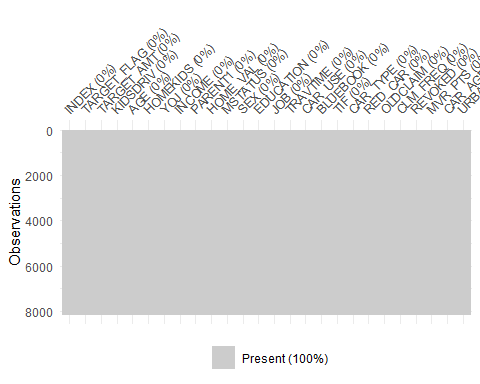
\includegraphics{Data621-Group1-HW3-FINAL_files/figure-latex/unnamed-chunk-15-1.pdf}

The plot on the right shows that the number of predictors with the
lowest BIC are \texttt{nox} , \texttt{age}, \texttt{rad}, and
\texttt{medv}. We will use those predictors to build the next model

\begin{longtable}[]{@{}ccccc@{}}
\toprule
\begin{minipage}[b]{0.21\columnwidth}\centering
~\strut
\end{minipage} & \begin{minipage}[b]{0.13\columnwidth}\centering
Estimate\strut
\end{minipage} & \begin{minipage}[b]{0.16\columnwidth}\centering
Std. Error\strut
\end{minipage} & \begin{minipage}[b]{0.12\columnwidth}\centering
z value\strut
\end{minipage} & \begin{minipage}[b]{0.14\columnwidth}\centering
Pr(\textgreater\textbar z\textbar)\strut
\end{minipage}\tabularnewline
\midrule
\endhead
\begin{minipage}[t]{0.21\columnwidth}\centering
\textbf{(Intercept)}\strut
\end{minipage} & \begin{minipage}[t]{0.13\columnwidth}\centering
-17.63\strut
\end{minipage} & \begin{minipage}[t]{0.16\columnwidth}\centering
2.168\strut
\end{minipage} & \begin{minipage}[t]{0.12\columnwidth}\centering
-8.131\strut
\end{minipage} & \begin{minipage}[t]{0.14\columnwidth}\centering
4.246e-16\strut
\end{minipage}\tabularnewline
\begin{minipage}[t]{0.21\columnwidth}\centering
\textbf{nox}\strut
\end{minipage} & \begin{minipage}[t]{0.13\columnwidth}\centering
23.62\strut
\end{minipage} & \begin{minipage}[t]{0.16\columnwidth}\centering
3.936\strut
\end{minipage} & \begin{minipage}[t]{0.12\columnwidth}\centering
6.003\strut
\end{minipage} & \begin{minipage}[t]{0.14\columnwidth}\centering
1.942e-09\strut
\end{minipage}\tabularnewline
\begin{minipage}[t]{0.21\columnwidth}\centering
\textbf{age}\strut
\end{minipage} & \begin{minipage}[t]{0.13\columnwidth}\centering
0.01824\strut
\end{minipage} & \begin{minipage}[t]{0.16\columnwidth}\centering
0.009172\strut
\end{minipage} & \begin{minipage}[t]{0.12\columnwidth}\centering
1.989\strut
\end{minipage} & \begin{minipage}[t]{0.14\columnwidth}\centering
0.04673\strut
\end{minipage}\tabularnewline
\begin{minipage}[t]{0.21\columnwidth}\centering
\textbf{rad}\strut
\end{minipage} & \begin{minipage}[t]{0.13\columnwidth}\centering
0.4528\strut
\end{minipage} & \begin{minipage}[t]{0.16\columnwidth}\centering
0.1093\strut
\end{minipage} & \begin{minipage}[t]{0.12\columnwidth}\centering
4.144\strut
\end{minipage} & \begin{minipage}[t]{0.14\columnwidth}\centering
3.413e-05\strut
\end{minipage}\tabularnewline
\begin{minipage}[t]{0.21\columnwidth}\centering
\textbf{medv}\strut
\end{minipage} & \begin{minipage}[t]{0.13\columnwidth}\centering
0.04481\strut
\end{minipage} & \begin{minipage}[t]{0.16\columnwidth}\centering
0.02319\strut
\end{minipage} & \begin{minipage}[t]{0.12\columnwidth}\centering
1.932\strut
\end{minipage} & \begin{minipage}[t]{0.14\columnwidth}\centering
0.05338\strut
\end{minipage}\tabularnewline
\bottomrule
\end{longtable}

(Dispersion parameter for binomial family taken to be 1 )

\begin{longtable}[]{@{}cc@{}}
\toprule
\endhead
\begin{minipage}[t]{0.27\columnwidth}\centering
Null deviance:\strut
\end{minipage} & \begin{minipage}[t]{0.37\columnwidth}\centering
645.9 on 465 degrees of freedom\strut
\end{minipage}\tabularnewline
\begin{minipage}[t]{0.27\columnwidth}\centering
Residual deviance:\strut
\end{minipage} & \begin{minipage}[t]{0.37\columnwidth}\centering
232.8 on 461 degrees of freedom\strut
\end{minipage}\tabularnewline
\bottomrule
\end{longtable}

\hypertarget{forward-selection-method-using-some-boxcox-transformed-independent-variables.-model-4}{%
\subsubsection{Forward Selection Method using some BoxCox transformed
independent variables. Model
4}\label{forward-selection-method-using-some-boxcox-transformed-independent-variables.-model-4}}

\begin{Shaded}
\begin{Highlighting}[]
\NormalTok{m4 <-}\StringTok{ }\KeywordTok{step}\NormalTok{(}\KeywordTok{glm}\NormalTok{(target}\OperatorTok{~}\DecValTok{1}\NormalTok{, }\DataTypeTok{data=}\NormalTok{crimeTrain), }\DataTypeTok{direction =} \StringTok{"forward"}\NormalTok{, }\DataTypeTok{scope =} \OperatorTok{~}\NormalTok{zn }\OperatorTok{+}\StringTok{ }\KeywordTok{I}\NormalTok{(}\KeywordTok{log}\NormalTok{(indus)) }\OperatorTok{+}\StringTok{ }\KeywordTok{I}\NormalTok{(}\KeywordTok{sqrt}\NormalTok{(chas)) }\OperatorTok{+}\StringTok{ }\KeywordTok{I}\NormalTok{(nox}\OperatorTok{^-}\DecValTok{1}\NormalTok{) }\OperatorTok{+}\StringTok{ }\KeywordTok{I}\NormalTok{(}\KeywordTok{log}\NormalTok{(rm)) }\OperatorTok{+}\StringTok{ }\KeywordTok{I}\NormalTok{(age}\OperatorTok{^}\DecValTok{2}\NormalTok{) }\OperatorTok{+}\StringTok{ }\KeywordTok{I}\NormalTok{(dis}\OperatorTok{^-}\NormalTok{.}\DecValTok{5}\NormalTok{) }\OperatorTok{+}\StringTok{ }\NormalTok{rad }\OperatorTok{+}\StringTok{ }\KeywordTok{I}\NormalTok{(tax}\OperatorTok{^-}\DecValTok{1}\NormalTok{) }\OperatorTok{+}\StringTok{ }\KeywordTok{I}\NormalTok{(ptratio}\OperatorTok{^}\DecValTok{2}\NormalTok{) }\OperatorTok{+}\StringTok{ }\NormalTok{lstat }\OperatorTok{+}\StringTok{ }\NormalTok{medv) }
\end{Highlighting}
\end{Shaded}

\begin{verbatim}
## Start:  AIC=680.3
## target ~ 1
## 
##                 Df Deviance    AIC
## + I(nox^-1)      1   50.349 291.51
## + I(age^2)       1   66.713 422.64
## + I(dis^-0.5)    1   66.801 423.26
## + rad            1   70.518 448.50
## + I(log(indus))  1   74.068 471.38
## + I(tax^-1)      1   74.547 474.39
## + lstat          1   90.834 566.47
## + zn             1   94.762 586.20
## + I(ptratio^2)   1  107.479 644.88
## + medv           1  107.941 646.88
## + I(log(rm))     1  112.912 667.86
## + I(sqrt(chas))  1  115.720 679.31
## <none>              116.466 680.30
## 
## Step:  AIC=291.51
## target ~ I(nox^-1)
## 
##                 Df Deviance    AIC
## + rad            1   45.272 243.97
## + I(tax^-1)      1   46.956 260.99
## + I(age^2)       1   49.650 286.99
## + I(ptratio^2)   1   49.778 288.19
## + I(log(rm))     1   49.876 289.10
## + medv           1   49.907 289.40
## + I(log(indus))  1   50.043 290.66
## <none>               50.349 291.51
## + zn             1   50.147 291.63
## + I(sqrt(chas))  1   50.305 293.10
## + lstat          1   50.336 293.38
## + I(dis^-0.5)    1   50.345 293.46
## 
## Step:  AIC=243.97
## target ~ I(nox^-1) + rad
## 
##                 Df Deviance    AIC
## + medv           1   44.061 233.33
## + I(age^2)       1   44.442 237.35
## + I(log(rm))     1   44.674 239.77
## + I(tax^-1)      1   45.017 243.34
## <none>               45.272 243.97
## + I(sqrt(chas))  1   45.113 244.33
## + lstat          1   45.149 244.71
## + I(dis^-0.5)    1   45.180 245.03
## + zn             1   45.223 245.47
## + I(ptratio^2)   1   45.240 245.64
## + I(log(indus))  1   45.267 245.92
## 
## Step:  AIC=233.33
## target ~ I(nox^-1) + rad + medv
## 
##                 Df Deviance    AIC
## + I(age^2)       1   43.027 224.27
## + I(tax^-1)      1   43.368 227.96
## + I(dis^-0.5)    1   43.827 232.86
## + lstat          1   43.834 232.93
## + I(log(indus))  1   43.856 233.17
## <none>               44.061 233.33
## + I(ptratio^2)   1   43.956 234.23
## + I(sqrt(chas))  1   44.030 235.01
## + I(log(rm))     1   44.052 235.24
## + zn             1   44.060 235.33
## 
## Step:  AIC=224.27
## target ~ I(nox^-1) + rad + medv + I(age^2)
## 
##                 Df Deviance    AIC
## + I(dis^-0.5)    1   42.184 217.05
## + I(tax^-1)      1   42.397 219.40
## <none>               43.027 224.27
## + I(log(indus))  1   42.888 224.77
## + I(ptratio^2)   1   42.975 225.71
## + I(sqrt(chas))  1   43.004 226.02
## + lstat          1   43.006 226.05
## + zn             1   43.013 226.12
## + I(log(rm))     1   43.024 226.24
## 
## Step:  AIC=217.05
## target ~ I(nox^-1) + rad + medv + I(age^2) + I(dis^-0.5)
## 
##                 Df Deviance    AIC
## + I(tax^-1)      1   41.399 210.29
## + I(log(indus))  1   41.866 215.53
## <none>               42.184 217.05
## + lstat          1   42.036 217.41
## + I(ptratio^2)   1   42.124 218.39
## + I(log(rm))     1   42.150 218.67
## + I(sqrt(chas))  1   42.169 218.89
## + zn             1   42.173 218.93
## 
## Step:  AIC=210.29
## target ~ I(nox^-1) + rad + medv + I(age^2) + I(dis^-0.5) + I(tax^-1)
## 
##                 Df Deviance    AIC
## + lstat          1   41.180 209.83
## <none>               41.399 210.29
## + I(log(indus))  1   41.232 210.42
## + I(ptratio^2)   1   41.318 211.38
## + I(log(rm))     1   41.360 211.86
## + I(sqrt(chas))  1   41.374 212.02
## + zn             1   41.396 212.27
## 
## Step:  AIC=209.83
## target ~ I(nox^-1) + rad + medv + I(age^2) + I(dis^-0.5) + I(tax^-1) + 
##     lstat
## 
##                 Df Deviance    AIC
## <none>               41.180 209.83
## + I(log(indus))  1   41.012 209.92
## + I(ptratio^2)   1   41.062 210.49
## + I(sqrt(chas))  1   41.159 211.59
## + zn             1   41.174 211.76
## + I(log(rm))     1   41.178 211.80
\end{verbatim}

\begin{Shaded}
\begin{Highlighting}[]
\KeywordTok{summary}\NormalTok{(m4)}
\end{Highlighting}
\end{Shaded}

\begin{verbatim}
## 
## Call:
## glm(formula = target ~ I(nox^-1) + rad + medv + I(age^2) + I(dis^-0.5) + 
##     I(tax^-1) + lstat, data = crimeTrain)
## 
## Deviance Residuals: 
##      Min        1Q    Median        3Q       Max  
## -0.70627  -0.18647  -0.02143   0.13160   0.98687  
## 
## Coefficients:
##               Estimate Std. Error t value Pr(>|t|)    
## (Intercept)  2.099e+00  2.682e-01   7.826 3.52e-14 ***
## I(nox^-1)   -8.407e-01  8.932e-02  -9.413  < 2e-16 ***
## rad          1.258e-02  2.698e-03   4.661 4.13e-06 ***
## medv         1.195e-02  2.464e-03   4.850 1.69e-06 ***
## I(age^2)     2.846e-05  7.544e-06   3.772 0.000183 ***
## I(dis^-0.5) -7.689e-01  2.123e-01  -3.621 0.000326 ***
## I(tax^-1)   -7.196e+01  2.332e+01  -3.086 0.002155 ** 
## lstat        5.686e-03  3.647e-03   1.559 0.119675    
## ---
## Signif. codes:  0 '***' 0.001 '**' 0.01 '*' 0.05 '.' 0.1 ' ' 1
## 
## (Dispersion parameter for gaussian family taken to be 0.08991273)
## 
##     Null deviance: 116.47  on 465  degrees of freedom
## Residual deviance:  41.18  on 458  degrees of freedom
## AIC: 209.83
## 
## Number of Fisher Scoring iterations: 2
\end{verbatim}

\hypertarget{select-models}{%
\section{SELECT MODELS}\label{select-models}}

\hypertarget{compare-model-statistics}{%
\subsection{Compare Model Statistics}\label{compare-model-statistics}}

\hypertarget{model-1---general-model}{%
\subsubsection{Model 1 - General Model}\label{model-1---general-model}}

\hypertarget{complete-general-model}{%
\paragraph{Complete general model}\label{complete-general-model}}

\textbf{ROC Curve}

The ROC Curve helps measure true positives and true negative. A high AUC
or area under the curve tells us the model is predicting well.

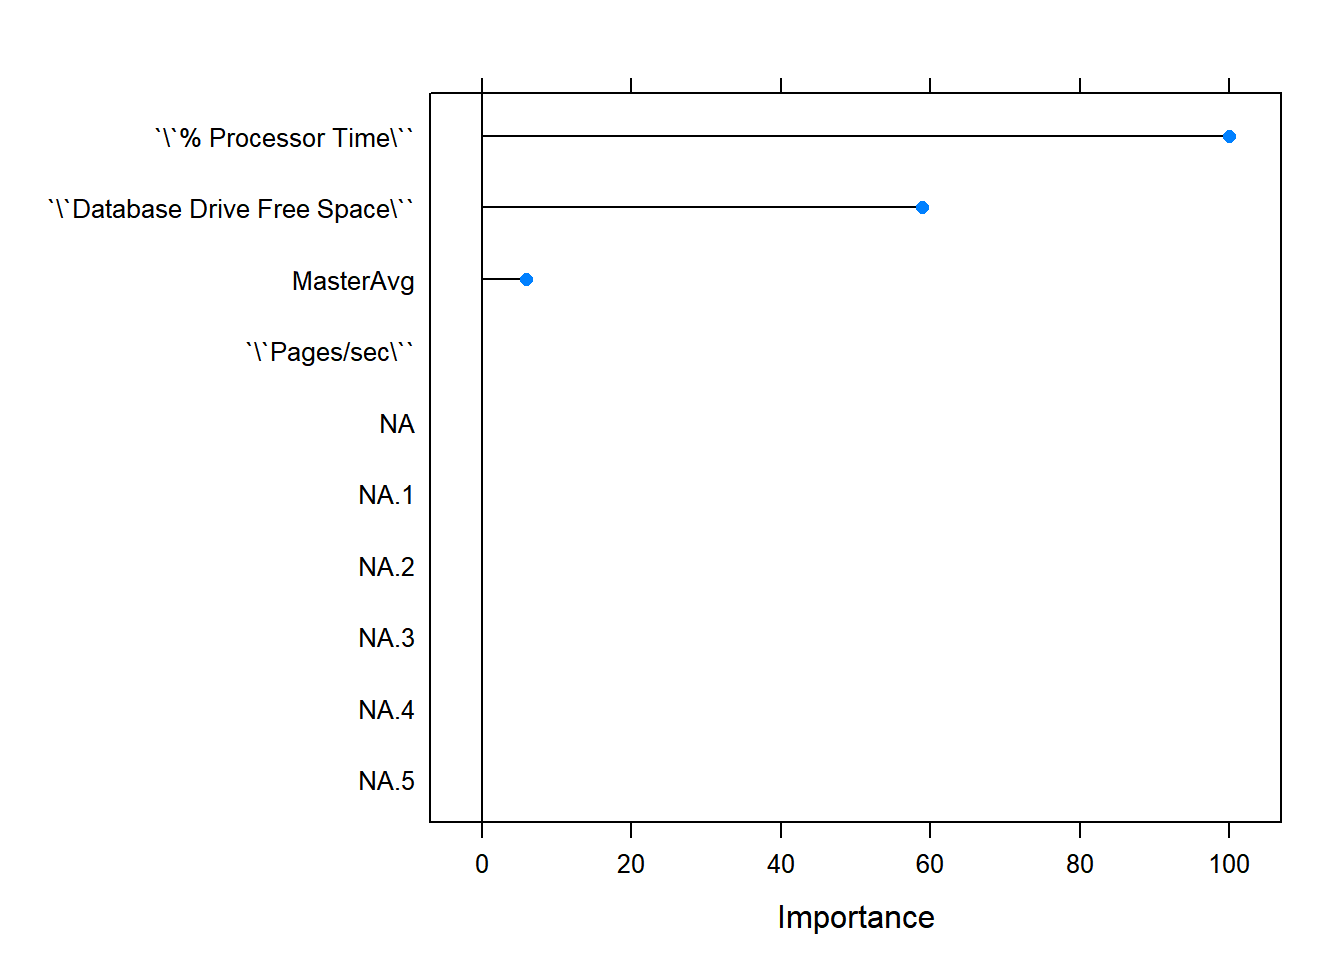
\includegraphics{Data621-Group1-HW3-FINAL_files/figure-latex/unnamed-chunk-18-1.pdf}

The AUC value of 0.97, tells us this model predicted values are acurate.

\textbf{Confusion Matrix}

\begin{verbatim}
##          
## targethat   0   1
##         0 220  22
##         1  17 207
\end{verbatim}

\textbf{Create a binned diagnostic plot of residuals vs prediction}
There are definite patterns here, which bear investigating.

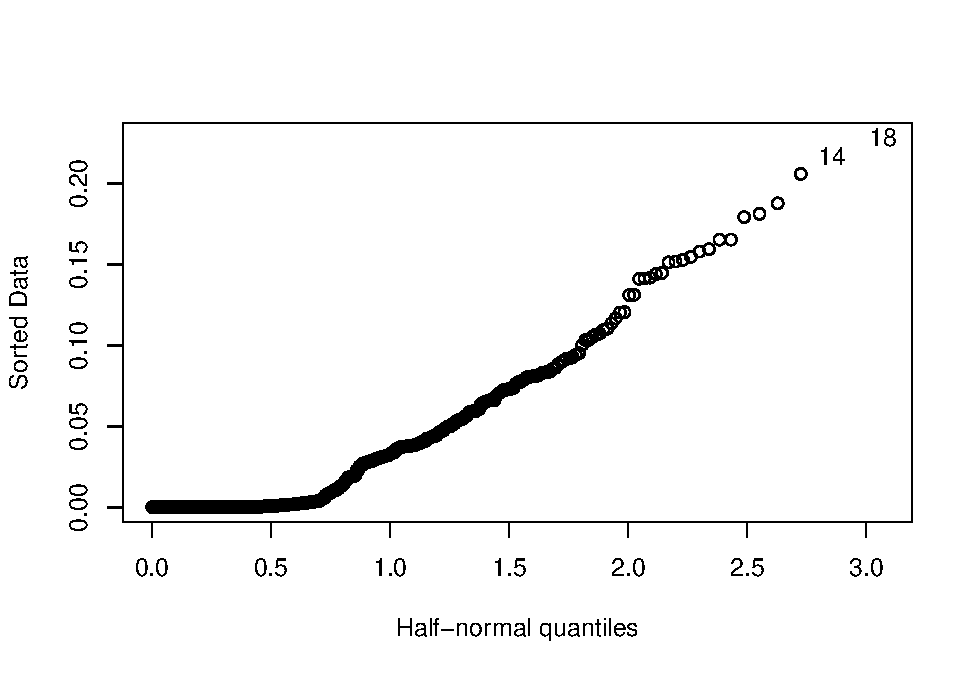
\includegraphics{Data621-Group1-HW3-FINAL_files/figure-latex/unnamed-chunk-20-1.pdf}

\textbf{Plot leverages.}

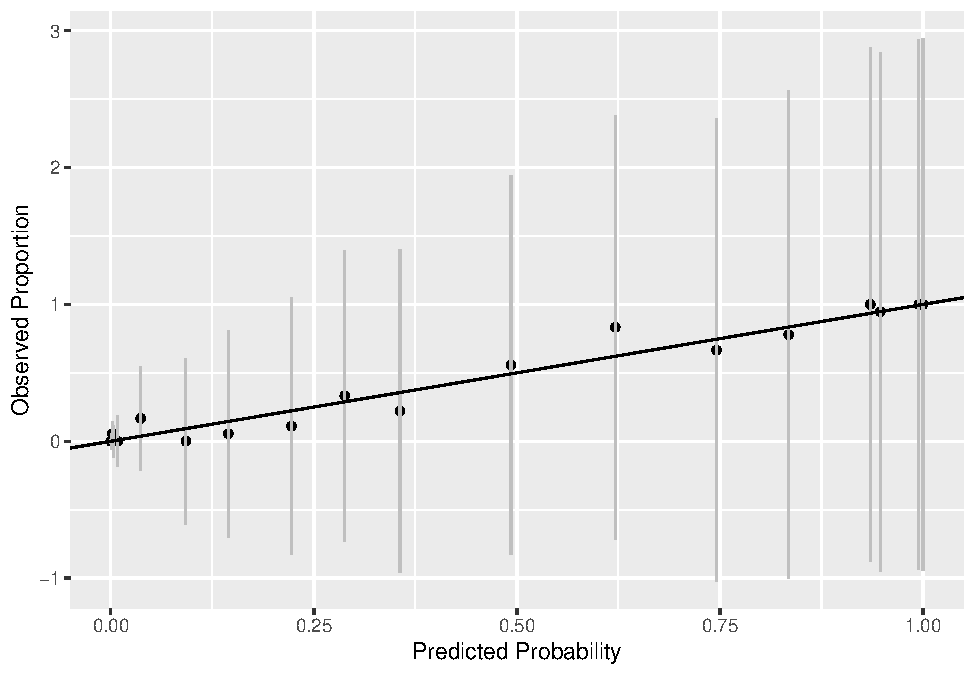
\includegraphics{Data621-Group1-HW3-FINAL_files/figure-latex/unnamed-chunk-21-1.pdf}

We don't see any strong outliers with the leverage plot. The points
identified (14,18) are essentially in the plot of the line formed, so
they are not likely pulling our model in any direction.

\textbf{Plot Goodness of fit}

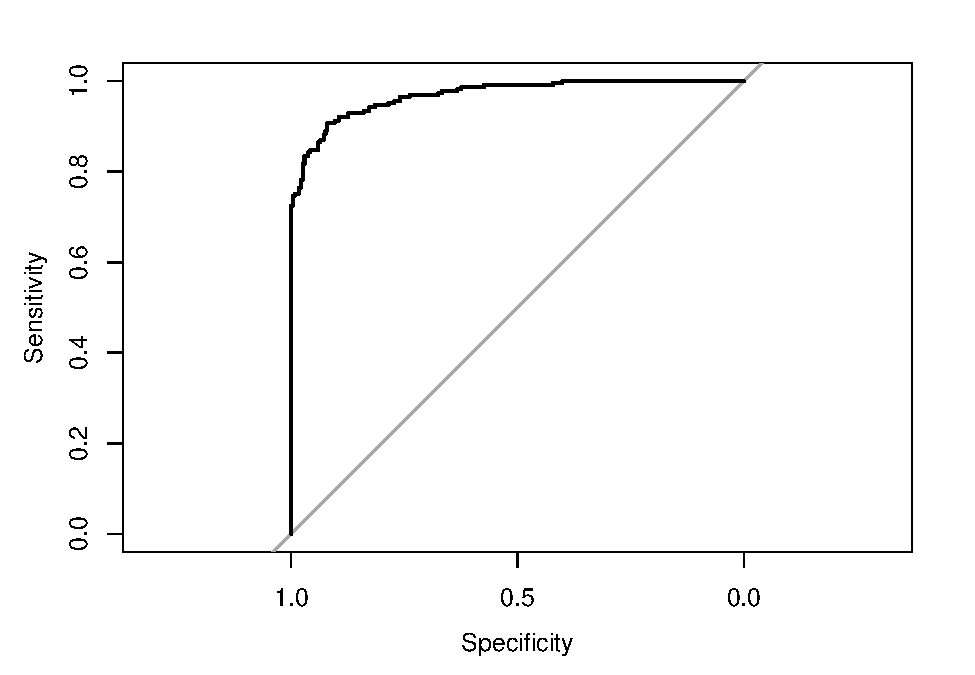
\includegraphics{Data621-Group1-HW3-FINAL_files/figure-latex/unnamed-chunk-22-1.pdf}

We see that our predictors fall close to the line.

\hypertarget{reduced-general-model}{%
\paragraph{Reduced general model}\label{reduced-general-model}}

\textbf{ROC Curve}
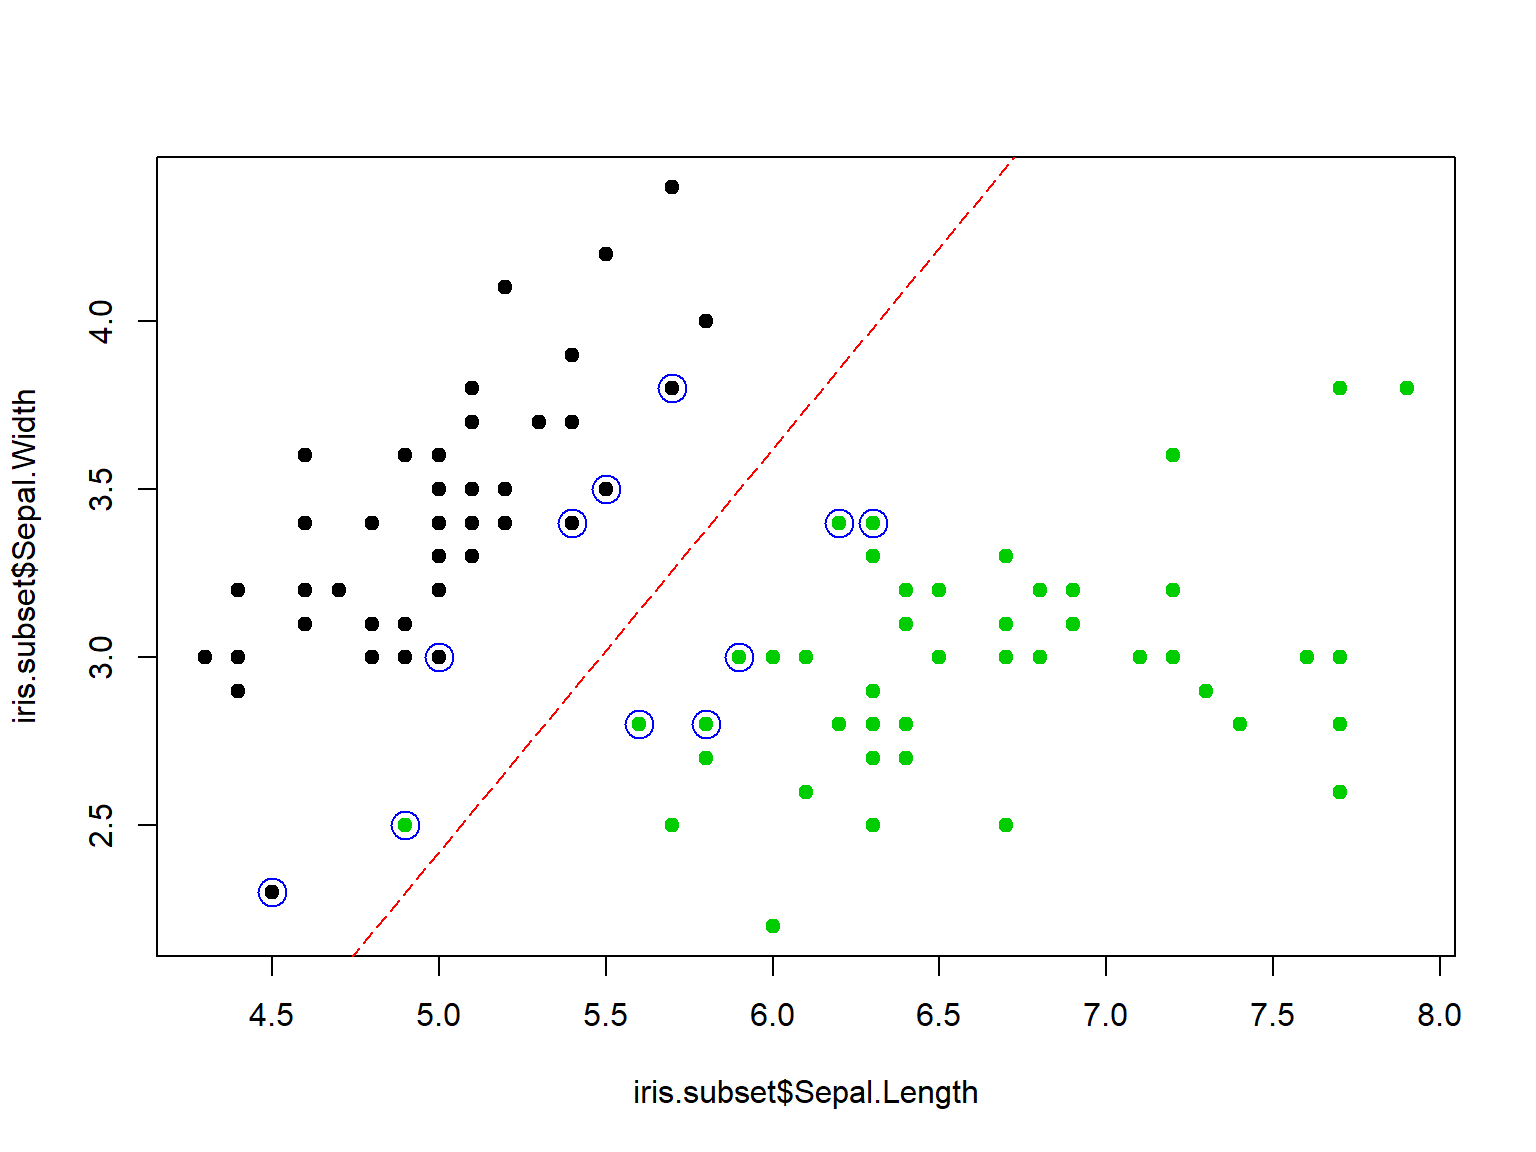
\includegraphics{Data621-Group1-HW3-FINAL_files/figure-latex/unnamed-chunk-23-1.pdf}

This model also show a high AUC value of 0.97. This tells us predicted
values are acurate, although slightly lower.

\textbf{Confusion Matrix}

\begin{verbatim}
##          
## targethat   0   1
##         0 218  22
##         1  19 207
\end{verbatim}

\textbf{Create a binned diagnostic plot of residuals vs prediction}
There are definite patterns here, which bear investigating.

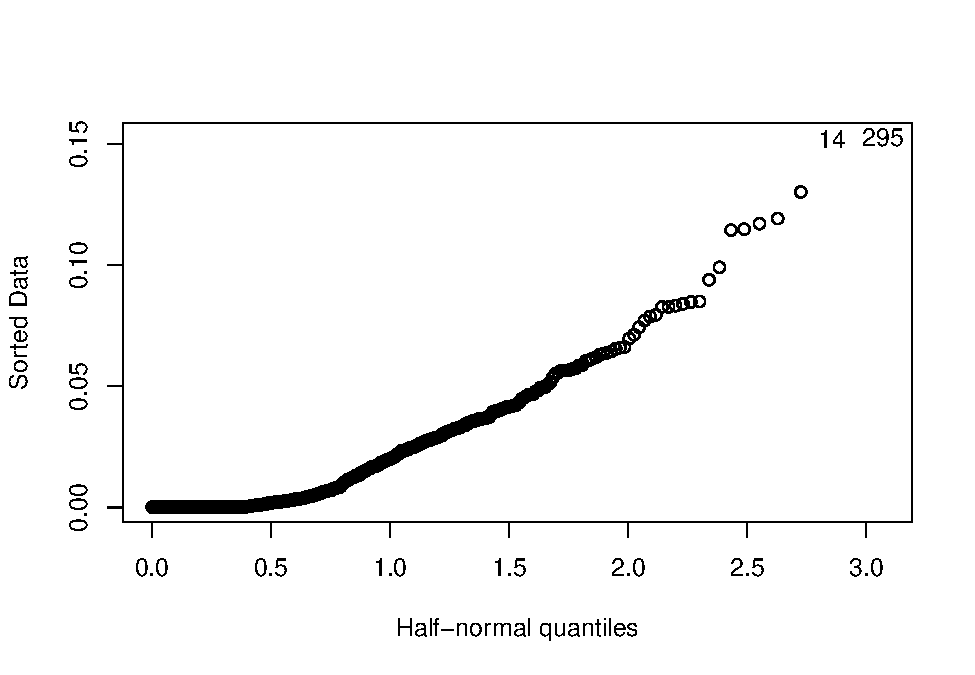
\includegraphics{Data621-Group1-HW3-FINAL_files/figure-latex/unnamed-chunk-25-1.pdf}

\textbf{Plot leverages.}

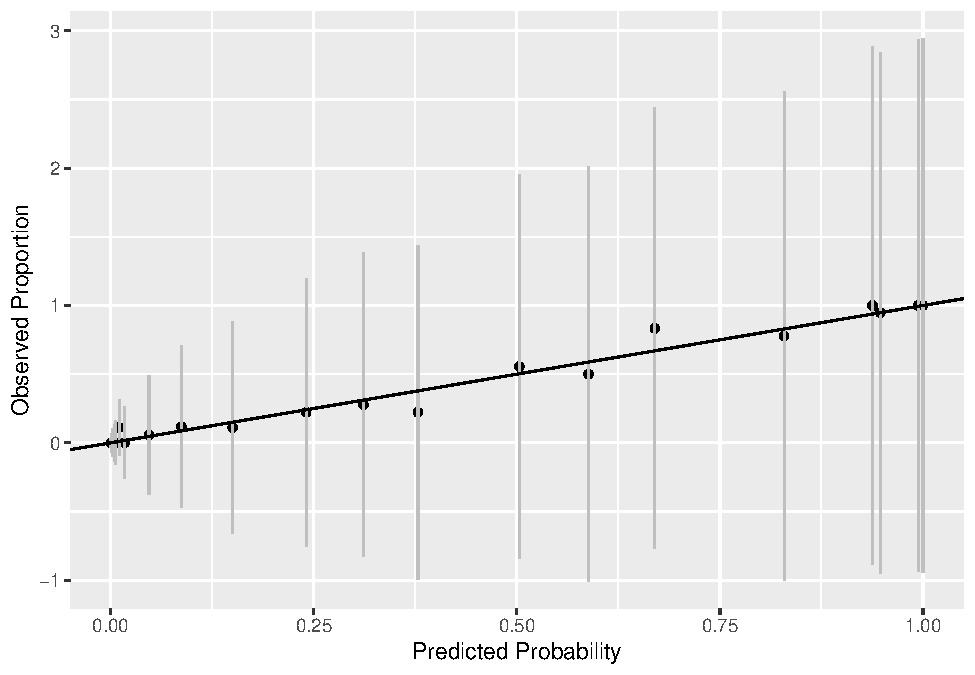
\includegraphics{Data621-Group1-HW3-FINAL_files/figure-latex/unnamed-chunk-26-1.pdf}

We don't see any strong outliers with the leverage plot. The points
identified (14,295) are essentially in the plot of the line formed, so
they are not likely pulling our model in any direction.

\textbf{Plot Goodness of fit}

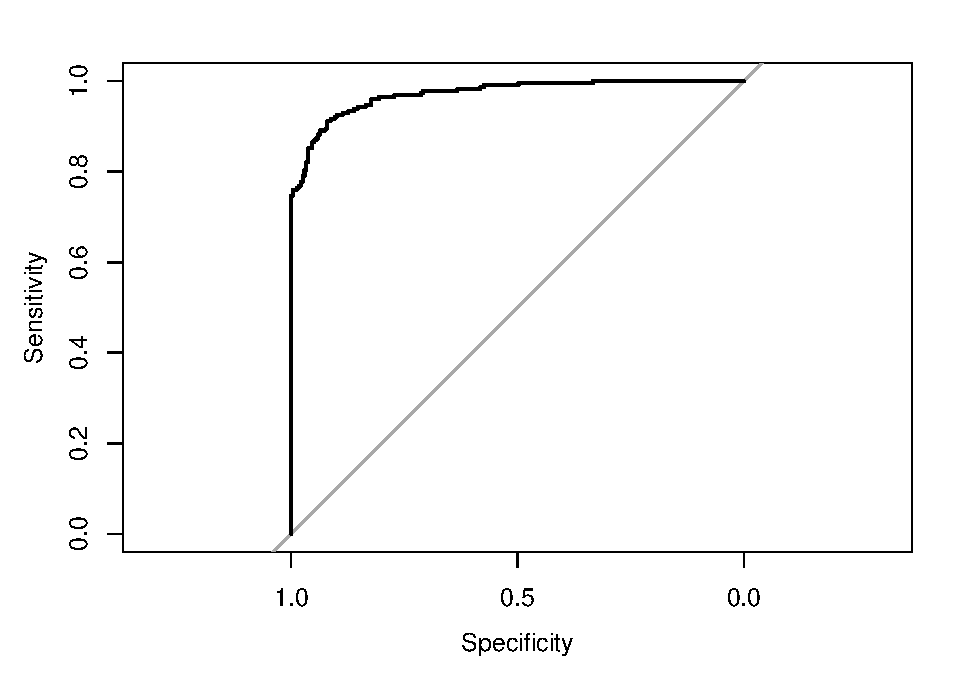
\includegraphics{Data621-Group1-HW3-FINAL_files/figure-latex/unnamed-chunk-27-1.pdf}

We see that our predictors fall close to the line.

\hypertarget{model-2---aic-model}{%
\subsubsection{Model 2 - AIC Model}\label{model-2---aic-model}}

\textbf{ROC Curve}
\includegraphics{Data621-Group1-HW3-FINAL_files/figure-latex/unnamed-chunk-28-1.pdf}

The AUC value of 0.97, tells us this model predicted values are acurate.

\textbf{Confusion Matrix}

\begin{verbatim}
##          
## targethat   0   1
##         0 218  22
##         1  19 207
\end{verbatim}

\textbf{Create a binned diagnostic plot of residuals vs prediction}

There seemes to be a slight pattern in the residuals for this model,
which may indicate the model isn't as good as we could get, but it
appears more random then the model 1 plot.

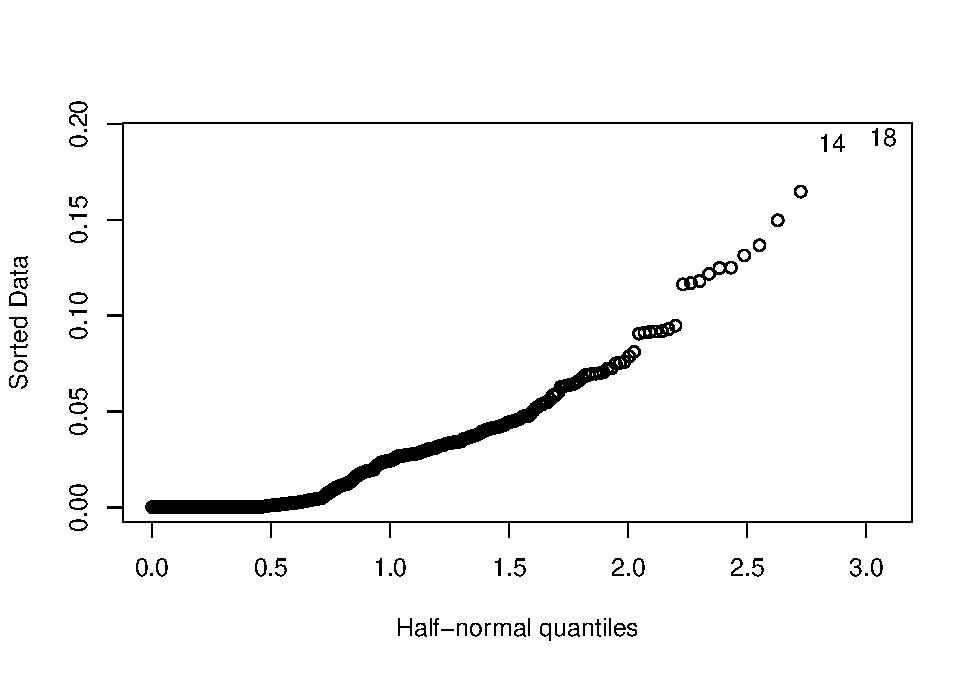
\includegraphics{Data621-Group1-HW3-FINAL_files/figure-latex/unnamed-chunk-30-1.pdf}

\textbf{Plot leverages.}

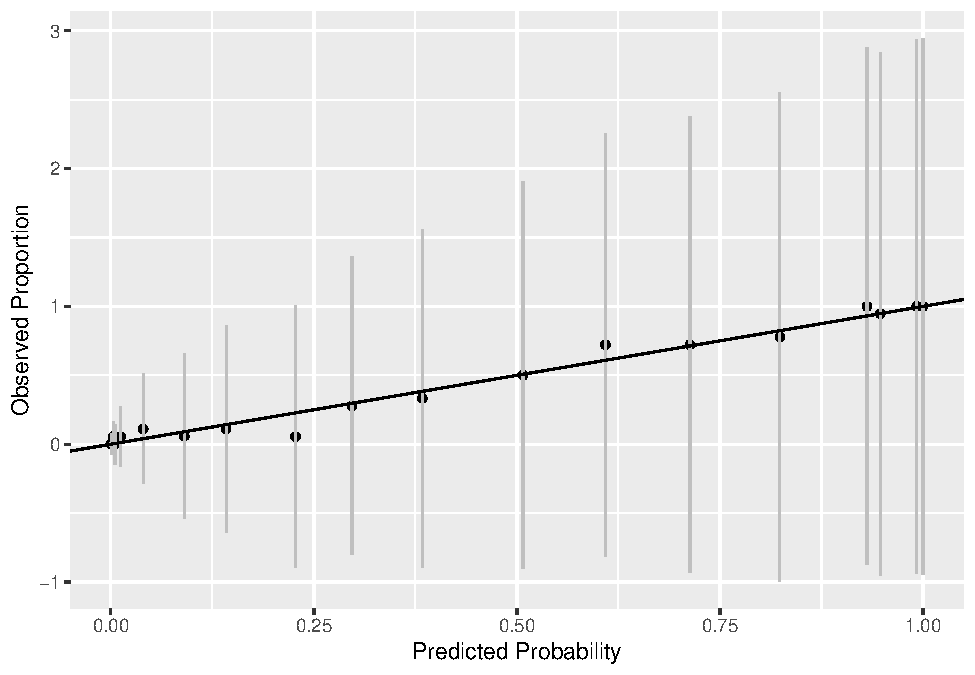
\includegraphics{Data621-Group1-HW3-FINAL_files/figure-latex/unnamed-chunk-31-1.pdf}

We don't see any strong outliers with the leverage plot. The points
identified (14,18) are essentially in the plot of the line formed, so
they are not likely pulling our model in any direction.

\textbf{Plot Goodness of fit}

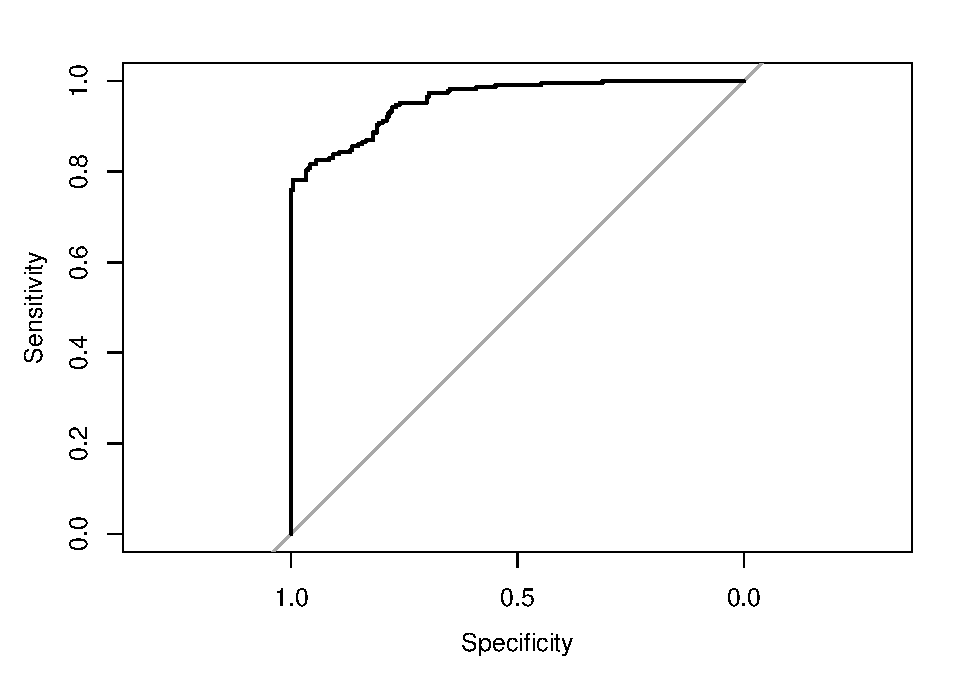
\includegraphics{Data621-Group1-HW3-FINAL_files/figure-latex/unnamed-chunk-32-1.pdf}

We see that our predictors fall close to the line.

\hypertarget{model-3---bic-model}{%
\subsubsection{Model 3 - BIC Model}\label{model-3---bic-model}}

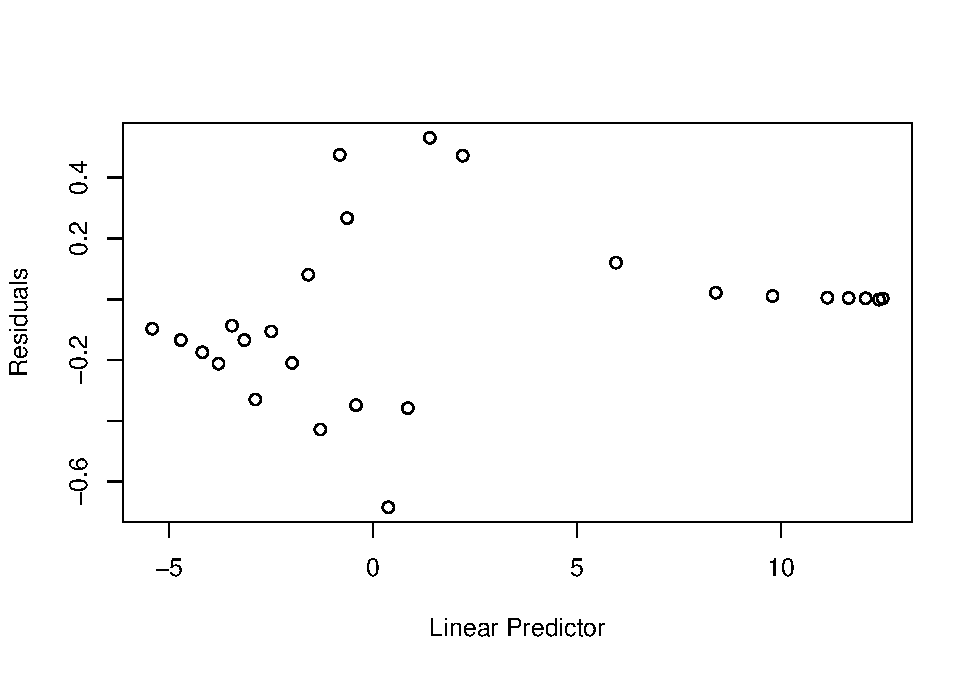
\includegraphics{Data621-Group1-HW3-FINAL_files/figure-latex/unnamed-chunk-33-1.pdf}

\begin{verbatim}
##          
## targethat   0   1
##         0 214  37
##         1  23 192
\end{verbatim}

The AUC value of 0.96, although high for this model it has the lowest
AUC score.

\textbf{Create a binned diagnostic plot of residuals vs prediction}

We see that the residuals plotted to the predictor seem less random than
in Model 2.

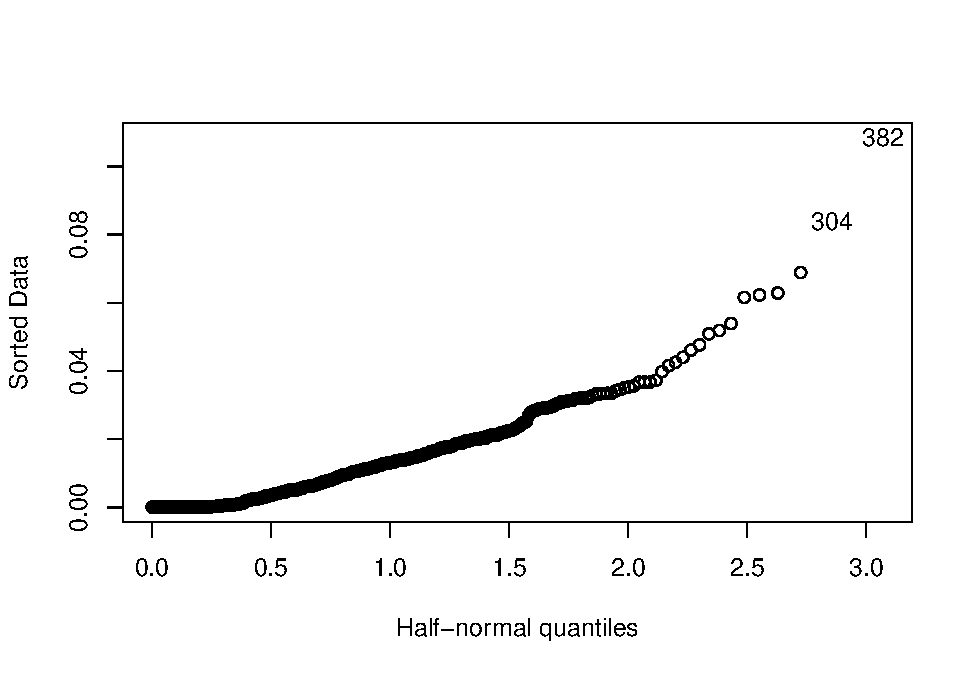
\includegraphics{Data621-Group1-HW3-FINAL_files/figure-latex/unnamed-chunk-34-1.pdf}

\textbf{Plot leverages.}

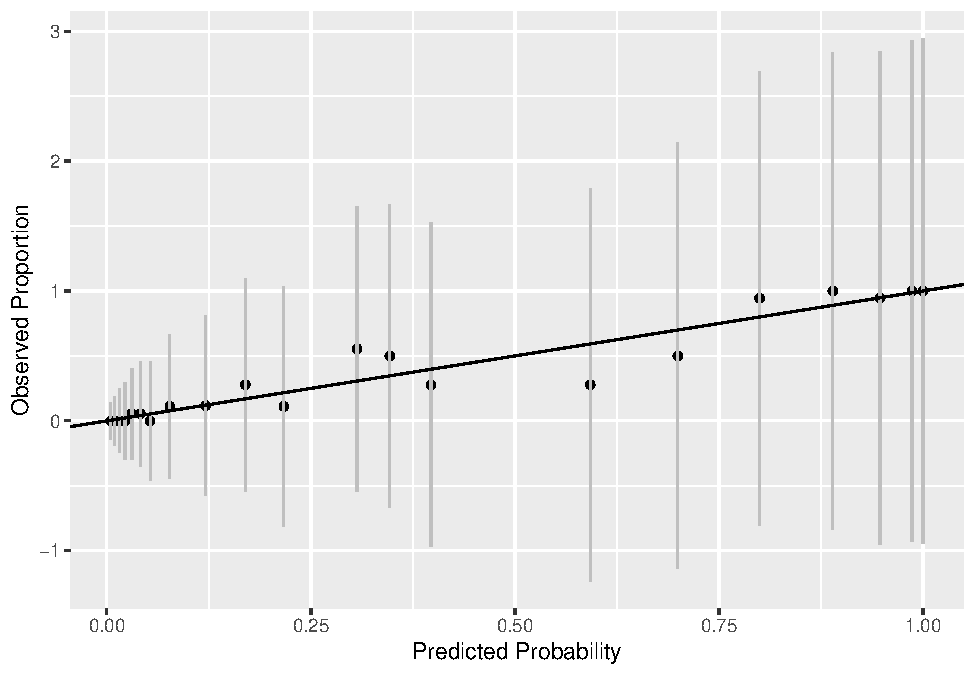
\includegraphics{Data621-Group1-HW3-FINAL_files/figure-latex/unnamed-chunk-35-1.pdf}

We don't see any strong outliers with the leverage plot. The points
identified (304,382) are essentially in the plot of the line formed, so
they are not likely pulling our model in any direction.

\textbf{Plot Goodness of fit}

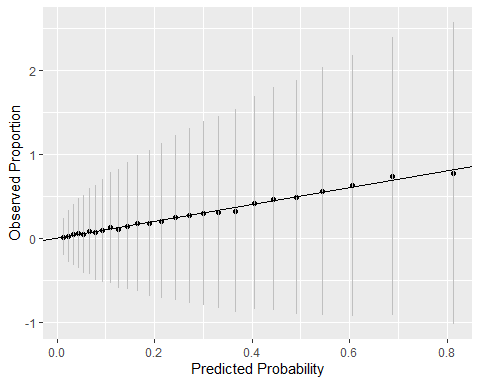
\includegraphics{Data621-Group1-HW3-FINAL_files/figure-latex/unnamed-chunk-36-1.pdf}

We see that our predictors fall close to the line.

\hypertarget{pick-the-best-regression-model}{%
\subsection{Pick the best regression
model}\label{pick-the-best-regression-model}}

\begin{longtable}[]{@{}lllll@{}}
\toprule
Metric & Model 1 & Model 2 & Model 3 & Model 4\tabularnewline
\midrule
\endhead
AIC & 218.0469179 & 215.3228528 & 242.7968243 &
209.8265226\tabularnewline
BIC & 271.9213312 & 252.6205235 & 263.5177525 &
247.1241933\tabularnewline
\bottomrule
\end{longtable}

From the above we see that Model 4, found by using the step forward
selection method to do stepwise reduction of models achieves both the
lowest AIC and the lowest BIC. Model 2 returns the next lowest metrics
and is the second best model from that evaluation criteria.

\hypertarget{conclusion}{%
\subsection{Conclusion}\label{conclusion}}

The final model selected with best AIC and BIC was model 4, which
includes a Box Cox transformation. The best logistic regression model
without transformation was model 2, with the lowest combination of AIC
and BIC. Both model 4 and model 2 were used to predict outcomes using
the evaluation data set.

When we did predictions with Model 4 we have found some results that
were confusing, as predictions should range between 0 and 1, and that
models predictions ranged somewhat above and below that. Because of that
we decided there is an error somewhere in that model causing erroneous
results and we will therefore use model 2 as our model selection and
hence use that to perform our predictions.

\textbf{Model 4 Evaluation}

\begin{verbatim}
##           1           2           3           4           5           6 
##  0.23290969  0.46707798  0.53401943  0.47377039  0.18116389  0.22707653 
##           7           8           9          10          11          12 
##  0.31726795  0.05238456 -0.01928392  0.02079947  0.36175503  0.31684788 
##          13          14          15          16          17          18 
##  0.62107178  0.68536094  0.66209469  0.37850731  0.28928192  0.64521511 
##          19          20          21          22          23          24 
##  0.13567823 -0.08554369 -0.28393681  0.14893165  0.27122208  0.23111746 
##          25          26          27          28          29          30 
##  0.20886975  0.26572067  0.04522059  1.10529854  1.14395035  0.80086859 
##          31          32          33          34          35          36 
##  1.10030433  1.12005903  1.08777600  1.21222859  1.12788637  1.10530173 
##          37          38          39          40 
##  1.15076375  1.01502028  0.54173080  0.41166762
\end{verbatim}

\textbf{Model 2 Evaluation}

\begin{verbatim}
##            1            2            3            4            5            6 
## 5.187335e-02 6.563639e-01 7.292303e-01 4.263767e-01 1.075746e-01 3.126897e-01 
##            7            8            9           10           11           12 
## 3.879178e-01 1.399105e-02 5.651298e-03 1.860232e-03 5.023729e-01 4.167837e-01 
##           13           14           15           16           17           18 
## 8.408851e-01 7.429792e-01 6.503036e-01 1.492647e-01 4.026110e-01 9.672516e-01 
##           19           20           21           22           23           24 
## 7.932839e-02 8.509218e-07 3.840253e-06 5.173182e-02 1.517637e-01 1.987527e-01 
##           25           26           27           28           29           30 
## 1.781289e-01 6.770735e-01 1.355059e-04 1.000000e+00 1.000000e+00 9.999947e-01 
##           31           32           33           34           35           36 
## 1.000000e+00 1.000000e+00 1.000000e+00 1.000000e+00 1.000000e+00 1.000000e+00 
##           37           38           39           40 
## 1.000000e+00 9.999999e-01 8.022854e-01 3.953354e-01
\end{verbatim}

For model 2 we can also use a threshold of 0.5, or 50\%, and compute the
binary prediction.

\begin{verbatim}
##  1  2  3  4  5  6  7  8  9 10 11 12 13 14 15 16 17 18 19 20 21 22 23 24 25 26 
##  0  1  1  0  0  0  0  0  0  0  1  0  1  1  1  0  0  1  0  0  0  0  0  0  0  1 
## 27 28 29 30 31 32 33 34 35 36 37 38 39 40 
##  0  1  1  1  1  1  1  1  1  1  1  1  1  0
\end{verbatim}

All models were computed using the entire training dataset. Because
models were selected using AIC and BIC metrics rather than evaluating
them using cross validation, the dataset was not initially split in
training and validate. Similar results are obtained performing this
split, as can be seen by reproducing model 2 with only 80\% of the
training set.

\begin{verbatim}
## Start:  AIC=218.05
## target ~ zn + indus + chas + nox + rm + age + dis + rad + tax + 
##     ptratio + lstat + medv
## 
##           Df Deviance    AIC
## - rm       1   192.71 216.71
## - lstat    1   192.77 216.77
## - chas     1   193.53 217.53
## - indus    1   193.99 217.99
## <none>         192.05 218.05
## - tax      1   196.59 220.59
## - zn       1   196.89 220.89
## - age      1   198.73 222.73
## - medv     1   199.95 223.95
## - ptratio  1   203.32 227.32
## - dis      1   203.84 227.84
## - rad      1   233.74 257.74
## - nox      1   265.05 289.05
## 
## Step:  AIC=216.71
## target ~ zn + indus + chas + nox + age + dis + rad + tax + ptratio + 
##     lstat + medv
## 
##           Df Deviance    AIC
## - chas     1   194.24 216.24
## - lstat    1   194.32 216.32
## - indus    1   194.58 216.58
## <none>         192.71 216.71
## - tax      1   197.59 219.59
## - zn       1   198.07 220.07
## - age      1   199.11 221.11
## - ptratio  1   203.53 225.53
## - dis      1   203.85 225.85
## - medv     1   205.35 227.35
## - rad      1   233.81 255.81
## - nox      1   265.14 287.14
## 
## Step:  AIC=216.24
## target ~ zn + indus + nox + age + dis + rad + tax + ptratio + 
##     lstat + medv
## 
##           Df Deviance    AIC
## - indus    1   195.51 215.51
## <none>         194.24 216.24
## - lstat    1   196.33 216.33
## - zn       1   200.59 220.59
## - tax      1   200.75 220.75
## - age      1   201.00 221.00
## - ptratio  1   203.94 223.94
## - dis      1   204.83 224.83
## - medv     1   207.12 227.12
## - rad      1   241.41 261.41
## - nox      1   265.19 285.19
## 
## Step:  AIC=215.51
## target ~ zn + nox + age + dis + rad + tax + ptratio + lstat + 
##     medv
## 
##           Df Deviance    AIC
## - lstat    1   197.32 215.32
## <none>         195.51 215.51
## - zn       1   202.05 220.05
## - age      1   202.23 220.23
## - ptratio  1   205.01 223.01
## - dis      1   205.96 223.96
## - tax      1   206.60 224.60
## - medv     1   208.13 226.13
## - rad      1   249.55 267.55
## - nox      1   270.59 288.59
## 
## Step:  AIC=215.32
## target ~ zn + nox + age + dis + rad + tax + ptratio + medv
## 
##           Df Deviance    AIC
## <none>         197.32 215.32
## - zn       1   203.45 219.45
## - ptratio  1   206.27 222.27
## - age      1   207.13 223.13
## - tax      1   207.62 223.62
## - dis      1   207.64 223.64
## - medv     1   208.65 224.65
## - rad      1   250.98 266.98
## - nox      1   273.18 289.18
\end{verbatim}

\begin{verbatim}
## 
## Call:
## glm(formula = target ~ zn + nox + age + dis + rad + tax + ptratio + 
##     medv, family = binomial(link = "logit"), data = crimeTrain)
## 
## Deviance Residuals: 
##     Min       1Q   Median       3Q      Max  
## -1.8295  -0.1752  -0.0021   0.0032   3.4191  
## 
## Coefficients:
##               Estimate Std. Error z value Pr(>|z|)    
## (Intercept) -37.415922   6.035013  -6.200 5.65e-10 ***
## zn           -0.068648   0.032019  -2.144  0.03203 *  
## nox          42.807768   6.678692   6.410 1.46e-10 ***
## age           0.032950   0.010951   3.009  0.00262 ** 
## dis           0.654896   0.214050   3.060  0.00222 ** 
## rad           0.725109   0.149788   4.841 1.29e-06 ***
## tax          -0.007756   0.002653  -2.924  0.00346 ** 
## ptratio       0.323628   0.111390   2.905  0.00367 ** 
## medv          0.110472   0.035445   3.117  0.00183 ** 
## ---
## Signif. codes:  0 '***' 0.001 '**' 0.01 '*' 0.05 '.' 0.1 ' ' 1
## 
## (Dispersion parameter for binomial family taken to be 1)
## 
##     Null deviance: 645.88  on 465  degrees of freedom
## Residual deviance: 197.32  on 457  degrees of freedom
## AIC: 215.32
## 
## Number of Fisher Scoring iterations: 9
\end{verbatim}

The final model preservers the predictors in the model with 100\% of the
training set. With the remaining 20\% we can also build a confusion
matrix, with similar results as seen in the analysis.

\begin{verbatim}
##          
## targethat  0  1
##         0 42  2
##         1  3 47
\end{verbatim}

\hypertarget{appendix}{%
\section{APPENDIX}\label{appendix}}

\begin{verbatim}
##    zn indus chas   nox    rm   age    dis rad tax ptratio lstat medv Target
## 1   0  7.07    0 0.469 7.185  61.1 4.9671   2 242    17.8  4.03 34.7      0
## 2   0  8.14    0 0.538 6.096  84.5 4.4619   4 307    21.0 10.26 18.2      1
## 3   0  8.14    0 0.538 6.495  94.4 4.4547   4 307    21.0 12.80 18.4      1
## 4   0  8.14    0 0.538 5.950  82.0 3.9900   4 307    21.0 27.71 13.2      0
## 5   0  5.96    0 0.499 5.850  41.5 3.9342   5 279    19.2  8.77 21.0      0
## 6  25  5.13    0 0.453 5.741  66.2 7.2254   8 284    19.7 13.15 18.7      0
## 7  25  5.13    0 0.453 5.966  93.4 6.8185   8 284    19.7 14.44 16.0      0
## 8   0  4.49    0 0.449 6.630  56.1 4.4377   3 247    18.5  6.53 26.6      0
## 9   0  4.49    0 0.449 6.121  56.8 3.7476   3 247    18.5  8.44 22.2      0
## 10  0  2.89    0 0.445 6.163  69.6 3.4952   2 276    18.0 11.34 21.4      0
## 11  0 25.65    0 0.581 5.856  97.0 1.9444   2 188    19.1 25.41 17.3      1
## 12  0 25.65    0 0.581 5.613  95.6 1.7572   2 188    19.1 27.26 15.7      0
## 13  0 21.89    0 0.624 5.637  94.7 1.9799   4 437    21.2 18.34 14.3      1
## 14  0 19.58    0 0.605 6.101  93.0 2.2834   5 403    14.7  9.81 25.0      1
## 15  0 19.58    0 0.605 5.880  97.3 2.3887   5 403    14.7 12.03 19.1      1
## 16  0 10.59    1 0.489 5.960  92.1 3.8771   4 277    18.6 17.27 21.7      0
## 17  0  6.20    0 0.504 6.552  21.4 3.3751   8 307    17.4  3.76 31.5      0
## 18  0  6.20    0 0.507 8.247  70.4 3.6519   8 307    17.4  3.95 48.3      1
## 19 22  5.86    0 0.431 6.957   6.8 8.9067   7 330    19.1  3.53 29.6      0
## 20 90  2.97    0 0.400 7.088  20.8 7.3073   1 285    15.3  7.85 32.2      0
## 21 80  1.76    0 0.385 6.230  31.5 9.0892   1 241    18.2 12.93 20.1      0
## 22 33  2.18    0 0.472 6.616  58.1 3.3700   7 222    18.4  8.93 28.4      0
## 23  0  9.90    0 0.544 6.122  52.8 2.6403   4 304    18.4  5.98 22.1      0
## 24  0  7.38    0 0.493 6.415  40.1 4.7211   5 287    19.6  6.12 25.0      0
## 25  0  7.38    0 0.493 6.312  28.9 5.4159   5 287    19.6  6.15 23.0      0
## 26  0  5.19    0 0.515 5.895  59.6 5.6150   5 224    20.2 10.56 18.5      1
## 27 80  2.01    0 0.435 6.635  29.7 8.3440   4 280    17.0  5.99 24.5      0
## 28  0 18.10    0 0.718 3.561  87.9 1.6132  24 666    20.2  7.12 27.5      1
## 29  0 18.10    1 0.631 7.016  97.5 1.2024  24 666    20.2  2.96 50.0      1
## 30  0 18.10    0 0.584 6.348  86.1 2.0527  24 666    20.2 17.64 14.5      1
## 31  0 18.10    0 0.740 5.935  87.9 1.8206  24 666    20.2 34.02  8.4      1
## 32  0 18.10    0 0.740 5.627  93.9 1.8172  24 666    20.2 22.88 12.8      1
## 33  0 18.10    0 0.740 5.818  92.4 1.8662  24 666    20.2 22.11 10.5      1
## 34  0 18.10    0 0.740 6.219 100.0 2.0048  24 666    20.2 16.59 18.4      1
## 35  0 18.10    0 0.740 5.854  96.6 1.8956  24 666    20.2 23.79 10.8      1
## 36  0 18.10    0 0.713 6.525  86.5 2.4358  24 666    20.2 18.13 14.1      1
## 37  0 18.10    0 0.713 6.376  88.4 2.5671  24 666    20.2 14.65 17.7      1
## 38  0 18.10    0 0.655 6.209  65.4 2.9634  24 666    20.2 13.22 21.4      1
## 39  0  9.69    0 0.585 5.794  70.6 2.8927   6 391    19.2 14.10 18.3      1
## 40  0 11.93    0 0.573 6.976  91.0 2.1675   1 273    21.0  5.64 23.9      0
\end{verbatim}

\textbf{Code used in analysis}

library(ggplot2) library(tidyr) library(MASS) library(psych)
library(kableExtra) library(dplyr) library(faraway) library(gridExtra)
library(reshape2) library(leaps) library(pROC) library(caret)
library(naniar) library(pander) library(pROC) crimeTrain \textless-
read.csv(``crime-training-data\_modified.csv'') crimeEval \textless-
read.csv(``crime-evaluation-data\_modified.csv'')

OVERVIEW

In this homework assignment, we will explore, analyze and model a data
set containing information on crime for various neighborhoods of a major
city. Each record has a response variable indicating whether or not the
crime rate is above the median crime rate (1) or not (0).

Objective:

The objective is to build a binary logistic regression model on the
training data set to predict whether the neighborhood will be at risk
for high crime levels.

DATA EXPLORATION

Data Summary

crimed1 \textless- describe(crimeTrain, na.rm = F)
crimed1\(na_count <- sapply(crimeTrain, function(y) sum(length(which(is.na(y))))) crimed1\)na\_count\_perc
\textless- sapply(crimeTrain, function(x)
round(sum(is.na(x))/nrow(crimeTrain)*100,1))

colsTrain\textless-ncol(crimeTrain) colsEval\textless-ncol(crimeEval)
missingCol\textless-colnames(crimeTrain){[}!(colnames(crimeTrain) \%in\%
colnames(crimeEval)){]}

The dataset consists of two data files: training and evaluation. The
training dataset contains 13 columns, while the evaluation dataset
contains 12. The evaluation dataset is missing column target which
represend our responce variable and defines whether the crime rate is
above the median crime rate (1) or not (0). We will start by exploring
the training data set since it will be the one used to generate the
regression model.

text\textless-``a test'' if(all(apply(crimeTrain,2,function(x)
is.numeric(x)))==TRUE) \{ text\textless-``all data is numeric'' \} else
\{ text\textless-``not all data is numeric'' \}
maxMeanMedianDiff\textless-round(max(abs(sapply(crimeTrain, median,
na.rm = T) - sapply(crimeTrain, mean, na.rm =
T))*100/(sapply(crimeTrain, max, na.rm = T)-sapply(crimeTrain, min,
na.rm = T))),2)

First we see that all data is numeric. The dataset does contain one
dummy variable to identify if the property borders the Charles River (1)
or not (0).

nas\textless-as.data.frame(sapply(crimeTrain, function(x)
sum(is.na(x)))) nasp\textless-as.data.frame(sapply(crimeTrain,
function(x) round(sum(is.na(x))/nrow(crimeTrain)\emph{100,1)))
colnames(nas)\textless-c(``name'') maxna\textless-max(nas)
maxnaname\textless-rownames(nas){[}nas\$name==maxna{]}
percent\textless-round(maxna/nrow(crimeTrain)}100,1)

An important aspect of any dataset is to determine how much, if any,
data is missing. We look at all the variables to see which if any have
missing data. We look at the basic descriptive statistics as well as the
missing data and their percentages:

kable(crimed1, ``html'', escape = F) \%\textgreater\%
kable\_styling(bootstrap\_options = c(``striped'', ``hover'',
``condensed''), full\_width = T) \%\textgreater\% column\_spec(1, bold =
T) \%\textgreater\% scroll\_box(width = ``100\%'', height = ``500px'')
sapply(crimeTrain, function(x)
round(sum(is.na(x))/nrow(crimeTrain)*100,1)) vis\_miss(crimeTrain)
head(crimeTrain)

Missing and Invalid Data

No missing data was found in the dataset.

With missing data assessed, we can look into the data in more detail. To
visualize this we plot histograms for each data. Several predictors like
dist, chas, rad, zn and tax are not normally distributed and noticable
outliers.

attach(crimeTrain{[},-1{]}) ggplot(gather(crimeTrain{[},-1{]}),
aes(value)) + geom\_histogram(bins = 20) +
facet\_wrap(\textasciitilde key, scales = ``free\_x'')
stripchart(data.frame(scale(crimeTrain)), method =``jitter'', las=2,
vertical=TRUE)

Mathematical transformations.

\textbf{Box Cox} The Box Cox transformation tries to transform
non-normal data into a normal distribution. This transformation attemps
to estimate the \(\lambda\) for Y. With the exception of tax, all
predictors have either no transformation extimate or were given a fudge
value of 0.

crimeTrain\_bct \textless- apply(crimeTrain, 2, BoxCoxTrans)
crimeTrain\_bct

Variable Creation / Removal

To determine how we can combine variables to create new one we start by
looking at a correlation plot. The plot and cor funtion lists nox, age,
rad,tax and indus as the strongest postively correlated predictors,
while rad and distance are the strongest negatively correlated
predictors. cor(crimeTrain\$target, crimeTrain{[}-c(1){]},
use=``na.or.complete'')

corrplot::corrplot(cor(crimeTrain{[},1:13{]}), order = ``hclust'',
method=`square', addrect = 2, tl.col = ``black'', tl.cex = .75, na.label
= " ")

BUILD MODELS

General regression

We start by building a model with all the predictors in the dataset.

m1\textless-glm(target\textasciitilde.,data=crimeTrain,family=``binomial''(link=``logit''))
summary(m1)

The Summary of this model shows several predictor are not relevant. We
build a second model without these predictors.

m1.1\textless-glm(target\textasciitilde nox+age+dis+rad+tax+ptratio+medv,data=crimeTrain,family=``binomial''(link=``logit''))
summary(m1.1)

1-pchisq(m1.1\(deviance,m1.1\)df.residual)
1-pchisq(m1\(deviance,m1\)df.residual)

The new model has a slightly higher AIC which would tells us the first
model is slightly less complex. For the 2 data sets p-value = 1 -
pchisq(deviance, degrees of freedom) are 1. The Null hypothesis is still
supported.

AIC Step Method Another way of selecting which predictors to use in the
model is by calculating the AIC of the model. This metric is similar to
the adjusted R-square of a model in that it penalizes models with more
predictors over simpler model with few predictors. We use Stepwise
function in r to find the lowest AIC with different predictors.

m2 \textless- step(m1) summary(m2)

This reduces the predictors used in the model to these: zn nox age dis
rad tax ptRation medv

It Removes these predictors: indus chas rm\#

The AIC improves marginally from 218.05 (our original general model) to
215.32, but we also benefit by having a simpler model less prone to
overfitting.

Also, the predictors in the model now are all signficant (under 0.05 pr
level) and all but one under .01 or very significant. Which is much
improved over the prior model

BIC Method

To determine the number of predictors and which predictors to be used we
will use the Bayesian Information Criterion (BIC).

regfit.full \textless- regsubsets(factor(target) \textasciitilde{} .,
data=crimeTrain) par(mfrow = c(1,2)) reg.summary \textless-
summary(regfit.full)
plot(reg.summary\(bic, xlab="Number of Predictors", ylab="BIC", type="l", main="Subset Selection Using BIC") BIC_num <- which.min(reg.summary\)bic)
points(BIC\_num, reg.summary\$bic{[}BIC\_num{]}, col=``red'', cex=2,
pch=20) plot(regfit.full, scale=``bic'', main=``Predictors vs.~BIC'')
par(mfrow = c(1,1))

The plot on the right shows that the number of predictors with the
lowest BIC are \texttt{nox} , \texttt{age}, \texttt{rad}, and
\texttt{medv}. We will use those predictors to build the next model

m3 \textless- glm(target \textasciitilde{} nox + age + rad + medv,
family=binomial, data = crimeTrain)
crimeTrain\(predicted_m3<- predict(m3, crimeTrain, type='response') crimeTrain\)target\_m3\(target <- ifelse(crimeTrain\)predicted\_m3\textgreater0.5,
1, 0) pander::pander(summary(m3))

Forward Selection Method using some BoxCox transformed independent
variables:

\{r\} m4 \textless- step(glm(target\textasciitilde1, data=crimeTrain),
direction = ``forward'', scope = \textasciitilde zn + I(log(indus)) +
I(sqrt(chas)) + I(nox\^{}-1) + I(log(rm)) + I(age\^{}2) + I(dis\^{}-.5)
+ rad + I(tax\^{}-1) + I(ptratio\^{}2) + lstat + medv) summary(m4)

SELECT MODELS Compare Model Statistics

Model 1 - General Model

Complete general model

\textbf{ROC Curve}

The ROC Curve helps measure true positives and true negative. A high AUC
or area under the curve tells us the model is predicting well.

targethat\textless-predict(m1,type=``response'')
g\textless-roc(target\textasciitilde targethat,data=crimeTrain) plot(g)

The AUC value of 0.96, tells us this model predicted values are acurate.

\textbf{Confusion Matrix}

targethat{[}targethat\textless0.5{]}\textless-0
targethat{[}targethat\textgreater=0.5{]}\textless-1
table(targethat,crimeTrain\$target)

\textbf{Create a binned diagnostic plot of residuals vs prediction}
There are definite patterns here, which bear investigating.

crimeMut \textless- mutate(crimeTrain, Residuals = residuals(m1),
linPred = predict(m1)) grpCrime \textless- group\_by(crimeMut,
cut(linPred, breaks=unique(quantile(linPred, (0:25/26))))) diagCrime
\textless- summarise(grpCrime, Residuals = mean(Residuals), linPred =
mean(linPred)) plot(Residuals \textasciitilde{} linPred, data =
diagCrime, xlab=``Linear Predictor'')

\textbf{Plot leverages.}

halfnorm(hatvalues(m1))

We don't see any strong outliers with the leverage plot. The points
identified (14,18) are essentially in the plot of the line formed, so
they are not likely pulling our model in any direction.

\textbf{Plot Goodness of fit}

linPred \textless- predict(m1) crimeMut \textless- mutate(crimeTrain,
predProb = predict(m1, type = ``response'')) grpCrime \textless-
group\_by(crimeMut, cut(linPred, breaks = unique(quantile(linPred,
(0:25)/26))))

hlDf \textless- summarise(grpCrime, y= sum(target),
pPred=mean(predProb), count = n()) hlDf \textless- mutate(hlDf,
se.fit=sqrt(pPred * (1-(pPred)/count)))
ggplot(hlDf,aes(x=pPred,y=y/count,ymin=y/count-2\emph{se.fit,ymax=y/count+2}se.fit))
+
geom\_point()+geom\_linerange(color=grey(0.75))+geom\_abline(intercept=0,slope=1)
+ xlab(``Predicted Probability'') + ylab(``Observed Proportion'')

We see that our predictors fall close to the line.

Reduced general model

\textbf{ROC Curve}

targethat\textless-predict(m1.1,type=``response'')
g\textless-roc(target\textasciitilde targethat,data=crimeTrain) plot(g)

This model also show a high AUC value of 0.96. This tells us predicted
values are acurate, although slightly lower.

\textbf{Confusion Matrix}

targethat{[}targethat\textless0.5{]}\textless-0
targethat{[}targethat\textgreater=0.5{]}\textless-1
table(targethat,crimeTrain\$target)

\textbf{Create a binned diagnostic plot of residuals vs prediction}
There are definite patterns here, which bear investigating.

crimeMut \textless- mutate(crimeTrain, Residuals = residuals(m1.1),
linPred = predict(m1.1)) grpCrime \textless- group\_by(crimeMut,
cut(linPred, breaks=unique(quantile(linPred, (0:25/26))))) diagCrime
\textless- summarise(grpCrime, Residuals = mean(Residuals), linPred =
mean(linPred)) plot(Residuals \textasciitilde{} linPred, data =
diagCrime, xlab=``Linear Predictor'')

\textbf{Plot leverages.}

halfnorm(hatvalues(m1.1))

We don't see any strong outliers with the leverage plot. The points
identified (14,18) are essentially in the plot of the line formed, so
they are not likely pulling our model in any direction.

\textbf{Plot Goodness of fit}

linPred \textless- predict(m1.1) crimeMut \textless- mutate(crimeTrain,
predProb = predict(m1.1, type = ``response'')) grpCrime \textless-
group\_by(crimeMut, cut(linPred, breaks = unique(quantile(linPred,
(0:25)/26))))

hlDf \textless- summarise(grpCrime, y= sum(target),
pPred=mean(predProb), count = n()) hlDf \textless- mutate(hlDf,
se.fit=sqrt(pPred * (1-(pPred)/count)))
ggplot(hlDf,aes(x=pPred,y=y/count,ymin=y/count-2\emph{se.fit,ymax=y/count+2}se.fit))
+
geom\_point()+geom\_linerange(color=grey(0.75))+geom\_abline(intercept=0,slope=1)
+ xlab(``Predicted Probability'') + ylab(``Observed Proportion'')

We see that our predictors fall close to the line.

Model 2 - AIC Model

\textbf{ROC Curve}

targethat\textless-predict(m2,type=``response'')
g\textless-roc(target\textasciitilde targethat,data=crimeTrain) plot(g)

The AUC value of 0.96, tells us this model predicted values are acurate.

\textbf{Confusion Matrix}

targethat{[}targethat\textless0.5{]}\textless-0
targethat{[}targethat\textgreater=0.5{]}\textless-1
table(targethat,crimeTrain\$target)

\textbf{Create a binned diagnostic plot of residuals vs prediction}

crimeMut \textless- mutate(crimeTrain, Residuals = residuals(m2),
linPred = predict(m2)) grpCrime \textless- group\_by(crimeMut,
cut(linPred, breaks=unique(quantile(linPred, (0:25/26))))) diagCrime
\textless- summarise(grpCrime, Residuals = mean(Residuals), linPred =
mean(linPred)) plot(Residuals \textasciitilde{} linPred, data =
diagCrime, xlab=``Linear Predictor'')

\textbf{Plot leverages.}

halfnorm(hatvalues(m2))

We don't see any strong outliers with the leverage plot. The points
identified (14,18) are essentially in the plot of the line formed, so
they are not likely pulling our model in any direction.

\textbf{Plot Goodness of fit}

linPred \textless- predict(m2) crimeMut \textless- mutate(crimeTrain,
predProb = predict(m2, type = ``response'')) grpCrime \textless-
group\_by(crimeMut, cut(linPred, breaks = unique(quantile(linPred,
(0:25)/26))))

hlDf \textless- summarise(grpCrime, y= sum(target),
pPred=mean(predProb), count = n()) hlDf \textless- mutate(hlDf,
se.fit=sqrt(pPred * (1-(pPred)/count)))
ggplot(hlDf,aes(x=pPred,y=y/count,ymin=y/count-2\emph{se.fit,ymax=y/count+2}se.fit))
+
geom\_point()+geom\_linerange(color=grey(0.75))+geom\_abline(intercept=0,slope=1)
+ xlab(``Predicted Probability'') + ylab(``Observed Proportion'')

We see that our predictors fall close to the line.

Model 3 - BIC Model

targethat\textless-predict(m3,type=``response'')
g\textless-roc(target\textasciitilde targethat,data=crimeTrain) plot(g)
targethat{[}targethat\textless0.5{]}\textless-0
targethat{[}targethat\textgreater=0.5{]}\textless-1
table(targethat,crimeTrain\$target)

The AUC value of 0.96, although high for this model it has the lowest
AUC score.

\textbf{Create a binned diagnostic plot of residuals vs prediction}

crimeMut \textless- mutate(crimeTrain, Residuals = residuals(m3),
linPred = predict(m3)) grpCrime \textless- group\_by(crimeMut,
cut(linPred, breaks=unique(quantile(linPred, (0:25/26))))) diagCrime
\textless- summarise(grpCrime, Residuals = mean(Residuals), linPred =
mean(linPred)) plot(Residuals \textasciitilde{} linPred, data =
diagCrime, xlab=``Linear Predictor'')

\textbf{Plot leverages.}

halfnorm(hatvalues(m3))

We don't see any strong outliers with the leverage plot. The points
identified (14,18) are essentially in the plot of the line formed, so
they are not likely pulling our model in any direction.

\textbf{Plot Goodness of fit}

linPred \textless- predict(m3) crimeMut \textless- mutate(crimeTrain,
predProb = predict(m3, type = ``response'')) grpCrime \textless-
group\_by(crimeMut, cut(linPred, breaks = unique(quantile(linPred,
(0:25)/26))))

hlDf \textless- summarise(grpCrime, y= sum(target),
pPred=mean(predProb), count = n()) hlDf \textless- mutate(hlDf,
se.fit=sqrt(pPred * (1-(pPred)/count)))
ggplot(hlDf,aes(x=pPred,y=y/count,ymin=y/count-2\emph{se.fit,ymax=y/count+2}se.fit))
+
geom\_point()+geom\_linerange(color=grey(0.75))+geom\_abline(intercept=0,slope=1)
+ xlab(``Predicted Probability'') + ylab(``Observed Proportion'')

We see that our predictors fall close to the line.

Pick the best regression model

m1AIC \textless- AIC(m1) m1BIC \textless- BIC(m1) m2AIC \textless-
AIC(m2) m2BIC \textless- BIC(m2) m3AIC \textless- AIC(m3) m3BIC
\textless- BIC(m3) m4AIC \textless- AIC(m4) m4BIC \textless- BIC(m4)
summary(m1)

\end{document}
